\documentclass[10pt,twocolumn]{article}
\usepackage[margin=0.8in]{geometry}
\usepackage{graphicx}
\usepackage{booktabs}
\usepackage{amsmath}
\usepackage{hyperref}
\usepackage{natbib}
% generated by analysis/make_claims.py
\expandafter\def\csname res@a4h_h4\endcsname{not confirmed}
\expandafter\def\csname res@a4hs_dform\endcsname{+0.04}
\expandafter\def\csname res@a4hs_dform_ci\endcsname{[+0.01, +0.09]}
\expandafter\def\csname res@a4hs_dhit\endcsname{+0.10}
\expandafter\def\csname res@a4hs_dhit_ci\endcsname{[+0.05, +0.15]}
\expandafter\def\csname res@a4hs_dj\endcsname{+0.04}
\expandafter\def\csname res@a4hs_dj_ci\endcsname{[-0.04, +0.12]}
\expandafter\def\csname res@a4hs_dj_p\endcsname{0.845}
\expandafter\def\csname res@a4hs_each_fa\endcsname{0.07}
\expandafter\def\csname res@a4hs_each_hit\endcsname{0.96}
\expandafter\def\csname res@a4hs_each_j\endcsname{+0.88}
\expandafter\def\csname res@a4hs_each_n\endcsname{136}
\expandafter\def\csname res@a4hs_iso_fa\endcsname{0.06}
\expandafter\def\csname res@a4hs_iso_hit\endcsname{0.90}
\expandafter\def\csname res@a4hs_iso_j\endcsname{+0.84}
\expandafter\def\csname res@a4hs_iso_n\endcsname{136}
\expandafter\def\csname res@a4hs_pick_fa\endcsname{0.12}
\expandafter\def\csname res@a4hs_pick_hit\endcsname{0.99}
\expandafter\def\csname res@a4hs_pick_j\endcsname{+0.88}
\expandafter\def\csname res@a4hs_pick_n\endcsname{136}
\expandafter\def\csname res@a4hu_dform\endcsname{+0.13}
\expandafter\def\csname res@a4hu_dform_ci\endcsname{[+0.01, +0.25]}
\expandafter\def\csname res@a4hu_dhit\endcsname{+0.18}
\expandafter\def\csname res@a4hu_dhit_ci\endcsname{[+0.09, +0.27]}
\expandafter\def\csname res@a4hu_dj\endcsname{-0.09}
\expandafter\def\csname res@a4hu_dj_ci\endcsname{[-0.26, +0.09]}
\expandafter\def\csname res@a4hu_dj_p\endcsname{0.170}
\expandafter\def\csname res@a4hu_each_fa\endcsname{0.45}
\expandafter\def\csname res@a4hu_each_hit\endcsname{0.57}
\expandafter\def\csname res@a4hu_each_j\endcsname{+0.12}
\expandafter\def\csname res@a4hu_each_n\endcsname{77}
\expandafter\def\csname res@a4hu_iso_fa\endcsname{0.32}
\expandafter\def\csname res@a4hu_iso_hit\endcsname{0.44}
\expandafter\def\csname res@a4hu_iso_j\endcsname{+0.12}
\expandafter\def\csname res@a4hu_iso_n\endcsname{78}
\expandafter\def\csname res@a4hu_pick_fa\endcsname{0.59}
\expandafter\def\csname res@a4hu_pick_hit\endcsname{0.62}
\expandafter\def\csname res@a4hu_pick_j\endcsname{+0.03}
\expandafter\def\csname res@a4hu_pick_n\endcsname{78}
\expandafter\def\csname res@a4s_h4\endcsname{not confirmed}
\expandafter\def\csname res@a4sens_hu_dj\endcsname{-0.14}
\expandafter\def\csname res@a4sens_hu_dj_ci\endcsname{[-0.36, +0.07]}
\expandafter\def\csname res@a4sens_hu_n\endcsname{56}
\expandafter\def\csname res@a4ss_dform\endcsname{+0.05}
\expandafter\def\csname res@a4ss_dform_ci\endcsname{[+0.01, +0.10]}
\expandafter\def\csname res@a4ss_dhit\endcsname{+0.06}
\expandafter\def\csname res@a4ss_dhit_ci\endcsname{[+0.01, +0.10]}
\expandafter\def\csname res@a4ss_dj\endcsname{+0.00}
\expandafter\def\csname res@a4ss_dj_ci\endcsname{[-0.07, +0.07]}
\expandafter\def\csname res@a4ss_dj_p\endcsname{0.539}
\expandafter\def\csname res@a4ss_each_fa\endcsname{0.09}
\expandafter\def\csname res@a4ss_each_hit\endcsname{0.94}
\expandafter\def\csname res@a4ss_each_j\endcsname{+0.85}
\expandafter\def\csname res@a4ss_each_n\endcsname{135}
\expandafter\def\csname res@a4ss_iso_fa\endcsname{0.08}
\expandafter\def\csname res@a4ss_iso_hit\endcsname{0.92}
\expandafter\def\csname res@a4ss_iso_j\endcsname{+0.84}
\expandafter\def\csname res@a4ss_iso_n\endcsname{134}
\expandafter\def\csname res@a4ss_pick_fa\endcsname{0.14}
\expandafter\def\csname res@a4ss_pick_hit\endcsname{0.98}
\expandafter\def\csname res@a4ss_pick_j\endcsname{+0.84}
\expandafter\def\csname res@a4ss_pick_n\endcsname{136}
\expandafter\def\csname res@a4su_dform\endcsname{+0.06}
\expandafter\def\csname res@a4su_dform_ci\endcsname{[-0.01, +0.14]}
\expandafter\def\csname res@a4su_dhit\endcsname{+0.29}
\expandafter\def\csname res@a4su_dhit_ci\endcsname{[+0.19, +0.41]}
\expandafter\def\csname res@a4su_dj\endcsname{+0.17}
\expandafter\def\csname res@a4su_dj_ci\endcsname{[+0.01, +0.32]}
\expandafter\def\csname res@a4su_dj_p\endcsname{0.986}
\expandafter\def\csname res@a4su_each_fa\endcsname{0.54}
\expandafter\def\csname res@a4su_each_hit\endcsname{0.65}
\expandafter\def\csname res@a4su_each_j\endcsname{+0.12}
\expandafter\def\csname res@a4su_each_n\endcsname{78}
\expandafter\def\csname res@a4su_iso_fa\endcsname{0.47}
\expandafter\def\csname res@a4su_iso_hit\endcsname{0.40}
\expandafter\def\csname res@a4su_iso_j\endcsname{-0.08}
\expandafter\def\csname res@a4su_iso_n\endcsname{78}
\expandafter\def\csname res@a4su_pick_fa\endcsname{0.60}
\expandafter\def\csname res@a4su_pick_hit\endcsname{0.69}
\expandafter\def\csname res@a4su_pick_j\endcsname{+0.09}
\expandafter\def\csname res@a4su_pick_n\endcsname{78}
\expandafter\def\csname res@a5_holm_H6\endcsname{1.000}
\expandafter\def\csname res@a5_holm_H7\endcsname{1.000}
\expandafter\def\csname res@a5_verdict_H6\endcsname{not confirmed}
\expandafter\def\csname res@a5_verdict_H7\endcsname{not confirmed}
\expandafter\def\csname res@a5s_dfa\endcsname{-0.01}
\expandafter\def\csname res@a5s_dfa_ci\endcsname{[-0.06, +0.04]}
\expandafter\def\csname res@a5s_dhit\endcsname{-0.02}
\expandafter\def\csname res@a5s_dhit_ci\endcsname{[-0.05, +0.00]}
\expandafter\def\csname res@a5s_dpauc\endcsname{-0.006}
\expandafter\def\csname res@a5s_dpauc_ci\endcsname{[-0.017, +0.011]}
\expandafter\def\csname res@a5s_fa_base\endcsname{0.11}
\expandafter\def\csname res@a5s_fa_pick\endcsname{0.12}
\expandafter\def\csname res@a5s_famax\endcsname{0.04}
\expandafter\def\csname res@a5s_n\endcsname{135}
\expandafter\def\csname res@a5sens_dpauc\endcsname{+0.001}
\expandafter\def\csname res@a5sens_dpauc_ci\endcsname{[-0.033, +0.047]}
\expandafter\def\csname res@a5u_dfa\endcsname{+0.01}
\expandafter\def\csname res@a5u_dfa_ci\endcsname{[-0.08, +0.12]}
\expandafter\def\csname res@a5u_dhit\endcsname{-0.04}
\expandafter\def\csname res@a5u_dhit_ci\endcsname{[-0.13, +0.05]}
\expandafter\def\csname res@a5u_dpauc\endcsname{+0.002}
\expandafter\def\csname res@a5u_dpauc_ci\endcsname{[-0.030, +0.045]}
\expandafter\def\csname res@a5u_fa_base\endcsname{0.60}
\expandafter\def\csname res@a5u_fa_pick\endcsname{0.59}
\expandafter\def\csname res@a5u_famax\endcsname{0.36}
\expandafter\def\csname res@a5u_n\endcsname{78}
\expandafter\def\csname res@al_hcs_each_a\endcsname{0.01}
\expandafter\def\csname res@al_hcs_each_chance\endcsname{0.02}
\expandafter\def\csname res@al_hcs_each_f\endcsname{0.07}
\expandafter\def\csname res@al_hcs_each_h\endcsname{0.97}
\expandafter\def\csname res@al_hcs_each_n\endcsname{143}
\expandafter\def\csname res@al_hcs_each_rate\endcsname{0.98}
\expandafter\def\csname res@al_hcs_each_sel\endcsname{0.99}
\expandafter\def\csname res@al_hcs_each_share\endcsname{0.92}
\expandafter\def\csname res@al_hcs_each_w\endcsname{0.02}
\expandafter\def\csname res@al_hcs_eif\endcsname{+0.01}
\expandafter\def\csname res@al_hcs_eif_ci\endcsname{[-0.02, +0.06]}
\expandafter\def\csname res@al_hcs_eih\endcsname{+0.05}
\expandafter\def\csname res@al_hcs_eih_ci\endcsname{[+0.01, +0.09]}
\expandafter\def\csname res@al_hcs_iso_a\endcsname{0.05}
\expandafter\def\csname res@al_hcs_iso_chance\endcsname{0.02}
\expandafter\def\csname res@al_hcs_iso_f\endcsname{0.06}
\expandafter\def\csname res@al_hcs_iso_h\endcsname{0.92}
\expandafter\def\csname res@al_hcs_iso_n\endcsname{143}
\expandafter\def\csname res@al_hcs_iso_rate\endcsname{0.97}
\expandafter\def\csname res@al_hcs_iso_sel\endcsname{0.95}
\expandafter\def\csname res@al_hcs_iso_share\endcsname{0.92}
\expandafter\def\csname res@al_hcs_iso_w\endcsname{0.03}
\expandafter\def\csname res@al_hcs_pef\endcsname{+0.06}
\expandafter\def\csname res@al_hcs_pef_ci\endcsname{[+0.01, +0.10]}
\expandafter\def\csname res@al_hcs_peh\endcsname{+0.03}
\expandafter\def\csname res@al_hcs_peh_ci\endcsname{[-0.00, +0.06]}
\expandafter\def\csname res@al_hcs_pick_a\endcsname{0.00}
\expandafter\def\csname res@al_hcs_pick_chance\endcsname{0.04}
\expandafter\def\csname res@al_hcs_pick_f\endcsname{0.13}
\expandafter\def\csname res@al_hcs_pick_h\endcsname{0.99}
\expandafter\def\csname res@al_hcs_pick_n\endcsname{143}
\expandafter\def\csname res@al_hcs_pick_rate\endcsname{0.99}
\expandafter\def\csname res@al_hcs_pick_sel\endcsname{1.00}
\expandafter\def\csname res@al_hcs_pick_share\endcsname{0.88}
\expandafter\def\csname res@al_hcs_pick_w\endcsname{0.01}
\expandafter\def\csname res@al_hcs_pif\endcsname{+0.07}
\expandafter\def\csname res@al_hcs_pif_ci\endcsname{[+0.02, +0.13]}
\expandafter\def\csname res@al_hcs_pih\endcsname{+0.07}
\expandafter\def\csname res@al_hcs_pih_ci\endcsname{[+0.03, +0.11]}
\expandafter\def\csname res@al_hcu_each_a\endcsname{0.24}
\expandafter\def\csname res@al_hcu_each_chance\endcsname{0.18}
\expandafter\def\csname res@al_hcu_each_f\endcsname{0.53}
\expandafter\def\csname res@al_hcu_each_h\endcsname{0.51}
\expandafter\def\csname res@al_hcu_each_n\endcsname{55}
\expandafter\def\csname res@al_hcu_each_rate\endcsname{0.67}
\expandafter\def\csname res@al_hcu_each_sel\endcsname{0.76}
\expandafter\def\csname res@al_hcu_each_share\endcsname{0.39}
\expandafter\def\csname res@al_hcu_each_w\endcsname{0.25}
\expandafter\def\csname res@al_hcu_eif\endcsname{+0.22}
\expandafter\def\csname res@al_hcu_eif_ci\endcsname{[+0.05, +0.38]}
\expandafter\def\csname res@al_hcu_eih\endcsname{+0.06}
\expandafter\def\csname res@al_hcu_eih_ci\endcsname{[-0.05, +0.18]}
\expandafter\def\csname res@al_hcu_iso_a\endcsname{0.38}
\expandafter\def\csname res@al_hcu_iso_chance\endcsname{0.10}
\expandafter\def\csname res@al_hcu_iso_f\endcsname{0.30}
\expandafter\def\csname res@al_hcu_iso_h\endcsname{0.44}
\expandafter\def\csname res@al_hcu_iso_n\endcsname{56}
\expandafter\def\csname res@al_hcu_iso_rate\endcsname{0.70}
\expandafter\def\csname res@al_hcu_iso_sel\endcsname{0.62}
\expandafter\def\csname res@al_hcu_iso_share\endcsname{0.47}
\expandafter\def\csname res@al_hcu_iso_w\endcsname{0.18}
\expandafter\def\csname res@al_hcu_pef\endcsname{+0.09}
\expandafter\def\csname res@al_hcu_pef_ci\endcsname{[-0.07, +0.24]}
\expandafter\def\csname res@al_hcu_peh\endcsname{+0.04}
\expandafter\def\csname res@al_hcu_peh_ci\endcsname{[-0.09, +0.16]}
\expandafter\def\csname res@al_hcu_pick_a\endcsname{0.18}
\expandafter\def\csname res@al_hcu_pick_chance\endcsname{0.21}
\expandafter\def\csname res@al_hcu_pick_f\endcsname{0.62}
\expandafter\def\csname res@al_hcu_pick_h\endcsname{0.54}
\expandafter\def\csname res@al_hcu_pick_n\endcsname{56}
\expandafter\def\csname res@al_hcu_pick_rate\endcsname{0.65}
\expandafter\def\csname res@al_hcu_pick_sel\endcsname{0.82}
\expandafter\def\csname res@al_hcu_pick_share\endcsname{0.37}
\expandafter\def\csname res@al_hcu_pick_w\endcsname{0.29}
\expandafter\def\csname res@al_hcu_pif\endcsname{+0.32}
\expandafter\def\csname res@al_hcu_pif_ci\endcsname{[+0.18, +0.46]}
\expandafter\def\csname res@al_hcu_pih\endcsname{+0.10}
\expandafter\def\csname res@al_hcu_pih_ci\endcsname{[+0.00, +0.19]}
\expandafter\def\csname res@al_hps_each_a\endcsname{0.01}
\expandafter\def\csname res@al_hps_each_chance\endcsname{0.02}
\expandafter\def\csname res@al_hps_each_f\endcsname{0.07}
\expandafter\def\csname res@al_hps_each_h\endcsname{0.97}
\expandafter\def\csname res@al_hps_each_n\endcsname{136}
\expandafter\def\csname res@al_hps_each_rate\endcsname{0.98}
\expandafter\def\csname res@al_hps_each_sel\endcsname{0.99}
\expandafter\def\csname res@al_hps_each_share\endcsname{0.91}
\expandafter\def\csname res@al_hps_each_w\endcsname{0.02}
\expandafter\def\csname res@al_hps_eif\endcsname{+0.01}
\expandafter\def\csname res@al_hps_eif_ci\endcsname{[-0.02, +0.06]}
\expandafter\def\csname res@al_hps_eih\endcsname{+0.05}
\expandafter\def\csname res@al_hps_eih_ci\endcsname{[+0.01, +0.09]}
\expandafter\def\csname res@al_hps_iso_a\endcsname{0.05}
\expandafter\def\csname res@al_hps_iso_chance\endcsname{0.02}
\expandafter\def\csname res@al_hps_iso_f\endcsname{0.06}
\expandafter\def\csname res@al_hps_iso_h\endcsname{0.92}
\expandafter\def\csname res@al_hps_iso_n\endcsname{136}
\expandafter\def\csname res@al_hps_iso_rate\endcsname{0.97}
\expandafter\def\csname res@al_hps_iso_sel\endcsname{0.95}
\expandafter\def\csname res@al_hps_iso_share\endcsname{0.91}
\expandafter\def\csname res@al_hps_iso_w\endcsname{0.03}
\expandafter\def\csname res@al_hps_pef\endcsname{+0.04}
\expandafter\def\csname res@al_hps_pef_ci\endcsname{[+0.01, +0.09]}
\expandafter\def\csname res@al_hps_peh\endcsname{+0.03}
\expandafter\def\csname res@al_hps_peh_ci\endcsname{[-0.00, +0.06]}
\expandafter\def\csname res@al_hps_pick_a\endcsname{0.00}
\expandafter\def\csname res@al_hps_pick_chance\endcsname{0.04}
\expandafter\def\csname res@al_hps_pick_f\endcsname{0.12}
\expandafter\def\csname res@al_hps_pick_h\endcsname{0.99}
\expandafter\def\csname res@al_hps_pick_n\endcsname{136}
\expandafter\def\csname res@al_hps_pick_rate\endcsname{0.99}
\expandafter\def\csname res@al_hps_pick_sel\endcsname{1.00}
\expandafter\def\csname res@al_hps_pick_share\endcsname{0.89}
\expandafter\def\csname res@al_hps_pick_w\endcsname{0.01}
\expandafter\def\csname res@al_hps_pif\endcsname{+0.06}
\expandafter\def\csname res@al_hps_pif_ci\endcsname{[+0.01, +0.11]}
\expandafter\def\csname res@al_hps_pih\endcsname{+0.07}
\expandafter\def\csname res@al_hps_pih_ci\endcsname{[+0.04, +0.12]}
\expandafter\def\csname res@al_hpu_each_a\endcsname{0.18}
\expandafter\def\csname res@al_hpu_each_chance\endcsname{0.15}
\expandafter\def\csname res@al_hpu_each_f\endcsname{0.45}
\expandafter\def\csname res@al_hpu_each_h\endcsname{0.59}
\expandafter\def\csname res@al_hpu_each_n\endcsname{77}
\expandafter\def\csname res@al_hpu_each_rate\endcsname{0.72}
\expandafter\def\csname res@al_hpu_each_sel\endcsname{0.82}
\expandafter\def\csname res@al_hpu_each_share\endcsname{0.47}
\expandafter\def\csname res@al_hpu_each_w\endcsname{0.23}
\expandafter\def\csname res@al_hpu_eif\endcsname{+0.13}
\expandafter\def\csname res@al_hpu_eif_ci\endcsname{[+0.00, +0.26]}
\expandafter\def\csname res@al_hpu_eih\endcsname{+0.06}
\expandafter\def\csname res@al_hpu_eih_ci\endcsname{[-0.03, +0.15]}
\expandafter\def\csname res@al_hpu_iso_a\endcsname{0.29}
\expandafter\def\csname res@al_hpu_iso_chance\endcsname{0.11}
\expandafter\def\csname res@al_hpu_iso_f\endcsname{0.32}
\expandafter\def\csname res@al_hpu_iso_h\endcsname{0.52}
\expandafter\def\csname res@al_hpu_iso_n\endcsname{78}
\expandafter\def\csname res@al_hpu_iso_rate\endcsname{0.74}
\expandafter\def\csname res@al_hpu_iso_sel\endcsname{0.71}
\expandafter\def\csname res@al_hpu_iso_share\endcsname{0.51}
\expandafter\def\csname res@al_hpu_iso_w\endcsname{0.18}
\expandafter\def\csname res@al_hpu_pef\endcsname{+0.13}
\expandafter\def\csname res@al_hpu_pef_ci\endcsname{[+0.01, +0.25]}
\expandafter\def\csname res@al_hpu_peh\endcsname{+0.03}
\expandafter\def\csname res@al_hpu_peh_ci\endcsname{[-0.07, +0.13]}
\expandafter\def\csname res@al_hpu_pick_a\endcsname{0.14}
\expandafter\def\csname res@al_hpu_pick_chance\endcsname{0.20}
\expandafter\def\csname res@al_hpu_pick_f\endcsname{0.59}
\expandafter\def\csname res@al_hpu_pick_h\endcsname{0.62}
\expandafter\def\csname res@al_hpu_pick_n\endcsname{78}
\expandafter\def\csname res@al_hpu_pick_rate\endcsname{0.72}
\expandafter\def\csname res@al_hpu_pick_sel\endcsname{0.86}
\expandafter\def\csname res@al_hpu_pick_share\endcsname{0.42}
\expandafter\def\csname res@al_hpu_pick_w\endcsname{0.24}
\expandafter\def\csname res@al_hpu_pif\endcsname{+0.27}
\expandafter\def\csname res@al_hpu_pif_ci\endcsname{[+0.14, +0.40]}
\expandafter\def\csname res@al_hpu_pih\endcsname{+0.09}
\expandafter\def\csname res@al_hpu_pih_ci\endcsname{[+0.02, +0.17]}
\expandafter\def\csname res@al_scs_each_a\endcsname{0.04}
\expandafter\def\csname res@al_scs_each_chance\endcsname{0.03}
\expandafter\def\csname res@al_scs_each_f\endcsname{0.08}
\expandafter\def\csname res@al_scs_each_h\endcsname{0.95}
\expandafter\def\csname res@al_scs_each_n\endcsname{142}
\expandafter\def\csname res@al_scs_each_rate\endcsname{0.99}
\expandafter\def\csname res@al_scs_each_sel\endcsname{0.96}
\expandafter\def\csname res@al_scs_each_share\endcsname{0.91}
\expandafter\def\csname res@al_scs_each_w\endcsname{0.01}
\expandafter\def\csname res@al_scs_eif\endcsname{+0.00}
\expandafter\def\csname res@al_scs_eif_ci\endcsname{[-0.05, +0.05]}
\expandafter\def\csname res@al_scs_eih\endcsname{+0.01}
\expandafter\def\csname res@al_scs_eih_ci\endcsname{[-0.02, +0.05]}
\expandafter\def\csname res@al_scs_iso_a\endcsname{0.02}
\expandafter\def\csname res@al_scs_iso_chance\endcsname{0.03}
\expandafter\def\csname res@al_scs_iso_f\endcsname{0.09}
\expandafter\def\csname res@al_scs_iso_h\endcsname{0.94}
\expandafter\def\csname res@al_scs_iso_n\endcsname{141}
\expandafter\def\csname res@al_scs_iso_rate\endcsname{0.96}
\expandafter\def\csname res@al_scs_iso_sel\endcsname{0.98}
\expandafter\def\csname res@al_scs_iso_share\endcsname{0.89}
\expandafter\def\csname res@al_scs_iso_w\endcsname{0.03}
\expandafter\def\csname res@al_scs_pef\endcsname{+0.06}
\expandafter\def\csname res@al_scs_pef_ci\endcsname{[+0.01, +0.11]}
\expandafter\def\csname res@al_scs_peh\endcsname{+0.04}
\expandafter\def\csname res@al_scs_peh_ci\endcsname{[+0.00, +0.07]}
\expandafter\def\csname res@al_scs_pick_a\endcsname{0.01}
\expandafter\def\csname res@al_scs_pick_chance\endcsname{0.05}
\expandafter\def\csname res@al_scs_pick_f\endcsname{0.14}
\expandafter\def\csname res@al_scs_pick_h\endcsname{0.99}
\expandafter\def\csname res@al_scs_pick_n\endcsname{143}
\expandafter\def\csname res@al_scs_pick_rate\endcsname{0.99}
\expandafter\def\csname res@al_scs_pick_sel\endcsname{0.99}
\expandafter\def\csname res@al_scs_pick_share\endcsname{0.87}
\expandafter\def\csname res@al_scs_pick_w\endcsname{0.01}
\expandafter\def\csname res@al_scs_pif\endcsname{+0.06}
\expandafter\def\csname res@al_scs_pif_ci\endcsname{[+0.00, +0.11]}
\expandafter\def\csname res@al_scs_pih\endcsname{+0.04}
\expandafter\def\csname res@al_scs_pih_ci\endcsname{[+0.01, +0.07]}
\expandafter\def\csname res@al_scu_each_a\endcsname{0.25}
\expandafter\def\csname res@al_scu_each_chance\endcsname{0.21}
\expandafter\def\csname res@al_scu_each_f\endcsname{0.62}
\expandafter\def\csname res@al_scu_each_h\endcsname{0.59}
\expandafter\def\csname res@al_scu_each_n\endcsname{56}
\expandafter\def\csname res@al_scu_each_rate\endcsname{0.79}
\expandafter\def\csname res@al_scu_each_sel\endcsname{0.75}
\expandafter\def\csname res@al_scu_each_share\endcsname{0.43}
\expandafter\def\csname res@al_scu_each_w\endcsname{0.16}
\expandafter\def\csname res@al_scu_eif\endcsname{+0.11}
\expandafter\def\csname res@al_scu_eif_ci\endcsname{[-0.04, +0.25]}
\expandafter\def\csname res@al_scu_eih\endcsname{+0.18}
\expandafter\def\csname res@al_scu_eih_ci\endcsname{[+0.08, +0.30]}
\expandafter\def\csname res@al_scu_iso_a\endcsname{0.30}
\expandafter\def\csname res@al_scu_iso_chance\endcsname{0.17}
\expandafter\def\csname res@al_scu_iso_f\endcsname{0.52}
\expandafter\def\csname res@al_scu_iso_h\endcsname{0.40}
\expandafter\def\csname res@al_scu_iso_n\endcsname{56}
\expandafter\def\csname res@al_scu_iso_rate\endcsname{0.58}
\expandafter\def\csname res@al_scu_iso_sel\endcsname{0.70}
\expandafter\def\csname res@al_scu_iso_share\endcsname{0.33}
\expandafter\def\csname res@al_scu_iso_w\endcsname{0.29}
\expandafter\def\csname res@al_scu_pef\endcsname{+0.04}
\expandafter\def\csname res@al_scu_pef_ci\endcsname{[-0.07, +0.14]}
\expandafter\def\csname res@al_scu_peh\endcsname{+0.02}
\expandafter\def\csname res@al_scu_peh_ci\endcsname{[-0.09, +0.12]}
\expandafter\def\csname res@al_scu_pick_a\endcsname{0.18}
\expandafter\def\csname res@al_scu_pick_chance\endcsname{0.22}
\expandafter\def\csname res@al_scu_pick_f\endcsname{0.66}
\expandafter\def\csname res@al_scu_pick_h\endcsname{0.61}
\expandafter\def\csname res@al_scu_pick_n\endcsname{56}
\expandafter\def\csname res@al_scu_pick_rate\endcsname{0.74}
\expandafter\def\csname res@al_scu_pick_sel\endcsname{0.82}
\expandafter\def\csname res@al_scu_pick_share\endcsname{0.41}
\expandafter\def\csname res@al_scu_pick_w\endcsname{0.21}
\expandafter\def\csname res@al_scu_pif\endcsname{+0.14}
\expandafter\def\csname res@al_scu_pif_ci\endcsname{[+0.02, +0.27]}
\expandafter\def\csname res@al_scu_pih\endcsname{+0.20}
\expandafter\def\csname res@al_scu_pih_ci\endcsname{[+0.08, +0.33]}
\expandafter\def\csname res@al_sps_each_a\endcsname{0.04}
\expandafter\def\csname res@al_sps_each_chance\endcsname{0.03}
\expandafter\def\csname res@al_sps_each_f\endcsname{0.09}
\expandafter\def\csname res@al_sps_each_h\endcsname{0.95}
\expandafter\def\csname res@al_sps_each_n\endcsname{135}
\expandafter\def\csname res@al_sps_each_rate\endcsname{0.98}
\expandafter\def\csname res@al_sps_each_sel\endcsname{0.96}
\expandafter\def\csname res@al_sps_each_share\endcsname{0.90}
\expandafter\def\csname res@al_sps_each_w\endcsname{0.01}
\expandafter\def\csname res@al_sps_eif\endcsname{+0.01}
\expandafter\def\csname res@al_sps_eif_ci\endcsname{[-0.04, +0.06]}
\expandafter\def\csname res@al_sps_eih\endcsname{+0.01}
\expandafter\def\csname res@al_sps_eih_ci\endcsname{[-0.03, +0.05]}
\expandafter\def\csname res@al_sps_iso_a\endcsname{0.02}
\expandafter\def\csname res@al_sps_iso_chance\endcsname{0.03}
\expandafter\def\csname res@al_sps_iso_f\endcsname{0.08}
\expandafter\def\csname res@al_sps_iso_h\endcsname{0.95}
\expandafter\def\csname res@al_sps_iso_n\endcsname{134}
\expandafter\def\csname res@al_sps_iso_rate\endcsname{0.97}
\expandafter\def\csname res@al_sps_iso_sel\endcsname{0.98}
\expandafter\def\csname res@al_sps_iso_share\endcsname{0.89}
\expandafter\def\csname res@al_sps_iso_w\endcsname{0.03}
\expandafter\def\csname res@al_sps_pef\endcsname{+0.05}
\expandafter\def\csname res@al_sps_pef_ci\endcsname{[+0.01, +0.10]}
\expandafter\def\csname res@al_sps_peh\endcsname{+0.03}
\expandafter\def\csname res@al_sps_peh_ci\endcsname{[-0.00, +0.07]}
\expandafter\def\csname res@al_sps_pick_a\endcsname{0.01}
\expandafter\def\csname res@al_sps_pick_chance\endcsname{0.05}
\expandafter\def\csname res@al_sps_pick_f\endcsname{0.14}
\expandafter\def\csname res@al_sps_pick_h\endcsname{0.98}
\expandafter\def\csname res@al_sps_pick_n\endcsname{136}
\expandafter\def\csname res@al_sps_pick_rate\endcsname{0.99}
\expandafter\def\csname res@al_sps_pick_sel\endcsname{0.99}
\expandafter\def\csname res@al_sps_pick_share\endcsname{0.86}
\expandafter\def\csname res@al_sps_pick_w\endcsname{0.01}
\expandafter\def\csname res@al_sps_pif\endcsname{+0.06}
\expandafter\def\csname res@al_sps_pif_ci\endcsname{[+0.01, +0.11]}
\expandafter\def\csname res@al_sps_pih\endcsname{+0.03}
\expandafter\def\csname res@al_sps_pih_ci\endcsname{[+0.00, +0.07]}
\expandafter\def\csname res@al_spu_each_a\endcsname{0.18}
\expandafter\def\csname res@al_spu_each_chance\endcsname{0.18}
\expandafter\def\csname res@al_spu_each_f\endcsname{0.54}
\expandafter\def\csname res@al_spu_each_h\endcsname{0.67}
\expandafter\def\csname res@al_spu_each_n\endcsname{78}
\expandafter\def\csname res@al_spu_each_rate\endcsname{0.82}
\expandafter\def\csname res@al_spu_each_sel\endcsname{0.82}
\expandafter\def\csname res@al_spu_each_share\endcsname{0.49}
\expandafter\def\csname res@al_spu_each_w\endcsname{0.15}
\expandafter\def\csname res@al_spu_eif\endcsname{+0.06}
\expandafter\def\csname res@al_spu_eif_ci\endcsname{[-0.04, +0.17]}
\expandafter\def\csname res@al_spu_eih\endcsname{+0.16}
\expandafter\def\csname res@al_spu_eih_ci\endcsname{[+0.08, +0.25]}
\expandafter\def\csname res@al_spu_iso_a\endcsname{0.23}
\expandafter\def\csname res@al_spu_iso_chance\endcsname{0.16}
\expandafter\def\csname res@al_spu_iso_f\endcsname{0.47}
\expandafter\def\csname res@al_spu_iso_h\endcsname{0.51}
\expandafter\def\csname res@al_spu_iso_n\endcsname{78}
\expandafter\def\csname res@al_spu_iso_rate\endcsname{0.66}
\expandafter\def\csname res@al_spu_iso_sel\endcsname{0.77}
\expandafter\def\csname res@al_spu_iso_share\endcsname{0.41}
\expandafter\def\csname res@al_spu_iso_w\endcsname{0.26}
\expandafter\def\csname res@al_spu_pef\endcsname{+0.06}
\expandafter\def\csname res@al_spu_pef_ci\endcsname{[-0.01, +0.14]}
\expandafter\def\csname res@al_spu_peh\endcsname{+0.02}
\expandafter\def\csname res@al_spu_peh_ci\endcsname{[-0.06, +0.10]}
\expandafter\def\csname res@al_spu_pick_a\endcsname{0.13}
\expandafter\def\csname res@al_spu_pick_chance\endcsname{0.20}
\expandafter\def\csname res@al_spu_pick_f\endcsname{0.60}
\expandafter\def\csname res@al_spu_pick_h\endcsname{0.69}
\expandafter\def\csname res@al_spu_pick_n\endcsname{78}
\expandafter\def\csname res@al_spu_pick_rate\endcsname{0.79}
\expandafter\def\csname res@al_spu_pick_sel\endcsname{0.87}
\expandafter\def\csname res@al_spu_pick_share\endcsname{0.47}
\expandafter\def\csname res@al_spu_pick_w\endcsname{0.18}
\expandafter\def\csname res@al_spu_pif\endcsname{+0.13}
\expandafter\def\csname res@al_spu_pif_ci\endcsname{[+0.03, +0.23]}
\expandafter\def\csname res@al_spu_pih\endcsname{+0.18}
\expandafter\def\csname res@al_spu_pih_ci\endcsname{[+0.09, +0.28]}
\expandafter\def\csname res@all_h_b\endcsname{+0.13}
\expandafter\def\csname res@all_h_b_ci\endcsname{[-0.04, +0.30]}
\expandafter\def\csname res@all_h_ds\endcsname{+0.07}
\expandafter\def\csname res@all_h_ds_ci\endcsname{[+0.01, +0.13]}
\expandafter\def\csname res@all_h_ns\endcsname{143}
\expandafter\def\csname res@all_s_b\endcsname{+0.03}
\expandafter\def\csname res@all_s_b_ci\endcsname{[-0.11, +0.17]}
\expandafter\def\csname res@all_s_ds\endcsname{+0.06}
\expandafter\def\csname res@all_s_ds_ci\endcsname{[+0.01, +0.11]}
\expandafter\def\csname res@all_s_ns\endcsname{141}
\expandafter\def\csname res@band_hi\endcsname{0.8}
\expandafter\def\csname res@band_lo\endcsname{0.2}
\expandafter\def\csname res@c2_conf_h1n\endcsname{24}
\expandafter\def\csname res@c2_conf_h2p\endcsname{0.043}
\expandafter\def\csname res@c2_haiku_all_gate\endcsname{passed}
\expandafter\def\csname res@c2_haiku_all_h1ci90\endcsname{[+0.04, +0.19]}
\expandafter\def\csname res@c2_haiku_all_h1d\endcsname{+0.12}
\expandafter\def\csname res@c2_haiku_all_h1eq\endcsname{not inside}
\expandafter\def\csname res@c2_haiku_all_h1n\endcsname{103}
\expandafter\def\csname res@c2_haiku_all_h2\endcsname{+0.12}
\expandafter\def\csname res@c2_haiku_all_h2ci\endcsname{[+0.04, +0.19]}
\expandafter\def\csname res@c2_haiku_all_h2p\endcsname{0.001}
\expandafter\def\csname res@c2_haiku_all_isowrong\endcsname{0.15}
\expandafter\def\csname res@c2_haiku_all_p1\endcsname{0.007}
\expandafter\def\csname res@c2_haiku_all_solve\endcsname{0.28}
\expandafter\def\csname res@c2_haiku_all_ta_iso\endcsname{0.30}
\expandafter\def\csname res@c2_haiku_all_ta_pick\endcsname{0.42}
\expandafter\def\csname res@c2_haiku_conf_gate\endcsname{failed}
\expandafter\def\csname res@c2_haiku_conf_h1ci90\endcsname{[-0.12, +0.12]}
\expandafter\def\csname res@c2_haiku_conf_h1d\endcsname{+0.00}
\expandafter\def\csname res@c2_haiku_conf_h1eq\endcsname{not inside}
\expandafter\def\csname res@c2_haiku_conf_h1n\endcsname{24}
\expandafter\def\csname res@c2_haiku_conf_h2\endcsname{+0.12}
\expandafter\def\csname res@c2_haiku_conf_h2ci\endcsname{[+0.00, +0.29]}
\expandafter\def\csname res@c2_haiku_conf_h2p\endcsname{0.043}
\expandafter\def\csname res@c2_haiku_conf_isowrong\endcsname{0.04}
\expandafter\def\csname res@c2_haiku_conf_solve\endcsname{0.88}
\expandafter\def\csname res@c2_haiku_conf_ta_iso\endcsname{0.12}
\expandafter\def\csname res@c2_haiku_conf_ta_pick\endcsname{0.12}
\expandafter\def\csname res@c2_haiku_repl_gate\endcsname{failed}
\expandafter\def\csname res@c2_haiku_repl_h1ci90\endcsname{[+0.06, +0.24]}
\expandafter\def\csname res@c2_haiku_repl_h1d\endcsname{+0.15}
\expandafter\def\csname res@c2_haiku_repl_h1eq\endcsname{not inside}
\expandafter\def\csname res@c2_haiku_repl_h1n\endcsname{79}
\expandafter\def\csname res@c2_haiku_repl_h2\endcsname{+0.11}
\expandafter\def\csname res@c2_haiku_repl_h2ci\endcsname{[+0.03, +0.20]}
\expandafter\def\csname res@c2_haiku_repl_h2p\endcsname{0.006}
\expandafter\def\csname res@c2_haiku_repl_isowrong\endcsname{0.18}
\expandafter\def\csname res@c2_haiku_repl_solve\endcsname{0.10}
\expandafter\def\csname res@c2_haiku_repl_ta_iso\endcsname{0.35}
\expandafter\def\csname res@c2_haiku_repl_ta_pick\endcsname{0.51}
\expandafter\def\csname res@c2_holm_haiku_H1\endcsname{0.621}
\expandafter\def\csname res@c2_holm_haiku_H2\endcsname{0.005}
\expandafter\def\csname res@c2_holm_sonnet_H1\endcsname{0.366}
\expandafter\def\csname res@c2_holm_sonnet_H2\endcsname{0.366}
\expandafter\def\csname res@c2_repl_h2\endcsname{+0.11}
\expandafter\def\csname res@c2_sonnet_conf_gate\endcsname{failed}
\expandafter\def\csname res@c2_sonnet_conf_h1ci90\endcsname{[-0.12, +0.12]}
\expandafter\def\csname res@c2_sonnet_conf_h1d\endcsname{+0.00}
\expandafter\def\csname res@c2_sonnet_conf_h1eq\endcsname{not inside}
\expandafter\def\csname res@c2_sonnet_conf_h1n\endcsname{17}
\expandafter\def\csname res@c2_sonnet_conf_h2\endcsname{+0.11}
\expandafter\def\csname res@c2_sonnet_conf_h2ci\endcsname{[+0.00, +0.26]}
\expandafter\def\csname res@c2_sonnet_conf_h2p\endcsname{0.122}
\expandafter\def\csname res@c2_sonnet_conf_isowrong\endcsname{0.03}
\expandafter\def\csname res@c2_sonnet_conf_solve\endcsname{0.92}
\expandafter\def\csname res@c2_sonnet_conf_ta_iso\endcsname{0.12}
\expandafter\def\csname res@c2_sonnet_conf_ta_pick\endcsname{0.12}
\expandafter\def\csname res@c2_sonnet_isoparse\endcsname{0.896}
\expandafter\def\csname res@c3_audit_mixed\endcsname{6}
\expandafter\def\csname res@c3_audit_solved\endcsname{14}
\expandafter\def\csname res@c3_disagree\endcsname{22}
\expandafter\def\csname res@c3_gate_diff\endcsname{0.10}
\expandafter\def\csname res@c3_gate_parse\endcsname{0.90}
\expandafter\def\csname res@c3_n_dup\endcsname{5}
\expandafter\def\csname res@c3_n_mixed\endcsname{50}
\expandafter\def\csname res@c3_n_solved\endcsname{137}
\expandafter\def\csname res@c3_n_ta\endcsname{278}
\expandafter\def\csname res@c3_n_unresolved\endcsname{1}
\expandafter\def\csname res@c3_n_unsolved\endcsname{90}
\expandafter\def\csname res@c3h_b\endcsname{+0.12}
\expandafter\def\csname res@c3h_b_ci\endcsname{[-0.03, +0.27]}
\expandafter\def\csname res@c3h_b_p\endcsname{0.065}
\expandafter\def\csname res@c3h_cost\endcsname{10.7}
\expandafter\def\csname res@c3h_ds\endcsname{+0.06}
\expandafter\def\csname res@c3h_ds_ci\endcsname{[+0.01, +0.11]}
\expandafter\def\csname res@c3h_ds_n\endcsname{137}
\expandafter\def\csname res@c3h_ds_p\endcsname{0.019}
\expandafter\def\csname res@c3h_du\endcsname{+0.24}
\expandafter\def\csname res@c3h_du_ci\endcsname{[+0.13, +0.36]}
\expandafter\def\csname res@c3h_du_n\endcsname{90}
\expandafter\def\csname res@c3h_du_p\endcsname{$<$0.001}
\expandafter\def\csname res@c3h_fam_arxiv\endcsname{+0.12}
\expandafter\def\csname res@c3h_fam_arxiv_ci\endcsname{[-0.04, +0.28]}
\expandafter\def\csname res@c3h_fam_arxiv_n\endcsname{140}
\expandafter\def\csname res@c3h_fam_arxiv_nu\endcsname{84}
\expandafter\def\csname res@c3h_fam_contest\endcsname{+0.11}
\expandafter\def\csname res@c3h_fam_contest_ci\endcsname{[-0.44, +0.66]}
\expandafter\def\csname res@c3h_fam_contest_n\endcsname{87}
\expandafter\def\csname res@c3h_fam_contest_nu\endcsname{6}
\expandafter\def\csname res@c3h_gate\endcsname{passed}
\expandafter\def\csname res@c3h_h2s\endcsname{+0.02}
\expandafter\def\csname res@c3h_h2s_ci\endcsname{[-0.01, +0.05]}
\expandafter\def\csname res@c3h_h2s_n\endcsname{137}
\expandafter\def\csname res@c3h_h2s_p\endcsname{0.128}
\expandafter\def\csname res@c3h_h2u\endcsname{+0.19}
\expandafter\def\csname res@c3h_h2u_ci\endcsname{[+0.11, +0.28]}
\expandafter\def\csname res@c3h_h2u_n\endcsname{90}
\expandafter\def\csname res@c3h_h2u_p\endcsname{$<$0.001}
\expandafter\def\csname res@c3h_holm_H1\endcsname{0.129}
\expandafter\def\csname res@c3h_holm_H1u\endcsname{$<$0.001}
\expandafter\def\csname res@c3h_holm_H2s\endcsname{0.129}
\expandafter\def\csname res@c3h_holm_H2u\endcsname{$<$0.001}
\expandafter\def\csname res@c3h_isoparse\endcsname{1.000}
\expandafter\def\csname res@c3h_isoright\endcsname{0.83}
\expandafter\def\csname res@c3h_isowrong\endcsname{0.08}
\expandafter\def\csname res@c3h_n\endcsname{227}
\expandafter\def\csname res@c3h_solved_iso\endcsname{0.06}
\expandafter\def\csname res@c3h_solved_pick\endcsname{0.12}
\expandafter\def\csname res@c3h_unadj\endcsname{+0.19}
\expandafter\def\csname res@c3h_unadj_ci\endcsname{[+0.06, +0.31]}
\expandafter\def\csname res@c3h_unsolved_iso\endcsname{0.36}
\expandafter\def\csname res@c3h_unsolved_pick\endcsname{0.60}
\expandafter\def\csname res@c3h_verdict_H1\endcsname{inconclusive}
\expandafter\def\csname res@c3h_verdict_H1u\endcsname{confirmed}
\expandafter\def\csname res@c3h_verdict_H2s\endcsname{inconclusive}
\expandafter\def\csname res@c3h_verdict_H2u\endcsname{confirmed}
\expandafter\def\csname res@c3s_b\endcsname{-0.02}
\expandafter\def\csname res@c3s_b_ci\endcsname{[-0.15, +0.11]}
\expandafter\def\csname res@c3s_b_p\endcsname{0.614}
\expandafter\def\csname res@c3s_cost\endcsname{66.2}
\expandafter\def\csname res@c3s_ds\endcsname{+0.06}
\expandafter\def\csname res@c3s_ds_ci\endcsname{[+0.01, +0.11]}
\expandafter\def\csname res@c3s_ds_n\endcsname{135}
\expandafter\def\csname res@c3s_ds_p\endcsname{0.021}
\expandafter\def\csname res@c3s_du\endcsname{+0.13}
\expandafter\def\csname res@c3s_du_ci\endcsname{[+0.04, +0.23]}
\expandafter\def\csname res@c3s_du_n\endcsname{90}
\expandafter\def\csname res@c3s_du_p\endcsname{0.004}
\expandafter\def\csname res@c3s_fam_arxiv\endcsname{-0.03}
\expandafter\def\csname res@c3s_fam_arxiv_ci\endcsname{[-0.17, +0.12]}
\expandafter\def\csname res@c3s_fam_arxiv_n\endcsname{140}
\expandafter\def\csname res@c3s_fam_arxiv_nu\endcsname{84}
\expandafter\def\csname res@c3s_fam_contest\endcsname{+0.05}
\expandafter\def\csname res@c3s_fam_contest_ci\endcsname{[-0.09, +0.18]}
\expandafter\def\csname res@c3s_fam_contest_n\endcsname{85}
\expandafter\def\csname res@c3s_fam_contest_nu\endcsname{6}
\expandafter\def\csname res@c3s_gate\endcsname{passed}
\expandafter\def\csname res@c3s_h2s\endcsname{+0.03}
\expandafter\def\csname res@c3s_h2s_ci\endcsname{[-0.01, +0.06]}
\expandafter\def\csname res@c3s_h2s_n\endcsname{135}
\expandafter\def\csname res@c3s_h2s_p\endcsname{0.076}
\expandafter\def\csname res@c3s_h2u\endcsname{+0.28}
\expandafter\def\csname res@c3s_h2u_ci\endcsname{[+0.18, +0.38]}
\expandafter\def\csname res@c3s_h2u_n\endcsname{90}
\expandafter\def\csname res@c3s_h2u_p\endcsname{$<$0.001}
\expandafter\def\csname res@c3s_holm_H1\endcsname{0.614}
\expandafter\def\csname res@c3s_holm_H1u\endcsname{0.012}
\expandafter\def\csname res@c3s_holm_H2s\endcsname{0.152}
\expandafter\def\csname res@c3s_holm_H2u\endcsname{$<$0.001}
\expandafter\def\csname res@c3s_isoparse\endcsname{1.000}
\expandafter\def\csname res@c3s_isoright\endcsname{0.86}
\expandafter\def\csname res@c3s_isowrong\endcsname{0.11}
\expandafter\def\csname res@c3s_n\endcsname{225}
\expandafter\def\csname res@c3s_solved_iso\endcsname{0.08}
\expandafter\def\csname res@c3s_solved_pick\endcsname{0.14}
\expandafter\def\csname res@c3s_unadj\endcsname{+0.07}
\expandafter\def\csname res@c3s_unadj_ci\endcsname{[-0.03, +0.18]}
\expandafter\def\csname res@c3s_unsolved_iso\endcsname{0.50}
\expandafter\def\csname res@c3s_unsolved_pick\endcsname{0.63}
\expandafter\def\csname res@c3s_verdict_H1\endcsname{inconclusive}
\expandafter\def\csname res@c3s_verdict_H1u\endcsname{confirmed}
\expandafter\def\csname res@c3s_verdict_H2s\endcsname{inconclusive}
\expandafter\def\csname res@c3s_verdict_H2u\endcsname{confirmed}
\expandafter\def\csname res@cal_haiku\endcsname{0.98}
\expandafter\def\csname res@cal_haiku_nowork\endcsname{0.97}
\expandafter\def\csname res@cal_sonnet\endcsname{0.93}
\expandafter\def\csname res@cal_sonnet_nowork\endcsname{0.95}
\expandafter\def\csname res@cli_version\endcsname{2.1.317}
\expandafter\def\csname res@cli_version_c3\endcsname{2.1.318}
\expandafter\def\csname res@cost_subjects\endcsname{283}
\expandafter\def\csname res@eq_margin\endcsname{0.10}
\expandafter\def\csname res@gm_cal\endcsname{0.38}
\expandafter\def\csname res@gm_ds\endcsname{+0.00}
\expandafter\def\csname res@gm_du\endcsname{+0.00}
\expandafter\def\csname res@gm_hu\endcsname{+0.10}
\expandafter\def\csname res@gm_isowrong\endcsname{0.80}
\expandafter\def\csname res@gm_n\endcsname{10}
\expandafter\def\csname res@h3_haiku_acc_haiku\endcsname{0.14}
\expandafter\def\csname res@h3_haiku_acc_sonnet\endcsname{0.16}
\expandafter\def\csname res@h3_haiku_ci\endcsname{[-0.04, +0.07]}
\expandafter\def\csname res@h3_haiku_d\endcsname{+0.02}
\expandafter\def\csname res@h3_haiku_n\endcsname{225}
\expandafter\def\csname res@h3_haiku_p\endcsname{0.294}
\expandafter\def\csname res@h3_sonnet_acc_haiku\endcsname{0.13}
\expandafter\def\csname res@h3_sonnet_acc_sonnet\endcsname{0.19}
\expandafter\def\csname res@h3_sonnet_ci\endcsname{[-0.01, +0.10]}
\expandafter\def\csname res@h3_sonnet_d\endcsname{+0.04}
\expandafter\def\csname res@h3_sonnet_n\endcsname{225}
\expandafter\def\csname res@h3_sonnet_p\endcsname{0.049}
\expandafter\def\csname res@h3_verdict\endcsname{inconclusive}
\expandafter\def\csname res@lab_n_garbled\endcsname{2}
\expandafter\def\csname res@lab_n_mislab\endcsname{5}
\expandafter\def\csname res@lab_n_pools\endcsname{7}
\expandafter\def\csname res@ledger_total\endcsname{86}
\expandafter\def\csname res@lvl90\endcsname{90\%}
\expandafter\def\csname res@lvl95\endcsname{95\%}
\expandafter\def\csname res@p1_gemma2_pickiso\endcsname{0.38}
\expandafter\def\csname res@p1_gemma2_pickiso_ci\endcsname{[+0.17, +0.59]}
\expandafter\def\csname res@p1_haiku_isowrong\endcsname{0.00}
\expandafter\def\csname res@p1_haiku_pick\endcsname{0.00}
\expandafter\def\csname res@p1_haiku_solve\endcsname{1.00}
\expandafter\def\csname res@p1_opus_isowrong\endcsname{0.00}
\expandafter\def\csname res@p1_opus_pick\endcsname{0.00}
\expandafter\def\csname res@p1_opus_solve\endcsname{1.00}
\expandafter\def\csname res@p1_sonnet_isowrong\endcsname{0.00}
\expandafter\def\csname res@p1_sonnet_pick\endcsname{0.00}
\expandafter\def\csname res@p1_sonnet_solve\endcsname{1.00}
\expandafter\def\csname res@p2_haiku_auroc\endcsname{0.64}
\expandafter\def\csname res@p2_sonnet_auroc\endcsname{0.59}
\expandafter\def\csname res@ph_all_ci\endcsname{[-0.01, +0.13]}
\expandafter\def\csname res@ph_all_d\endcsname{+0.06}
\expandafter\def\csname res@ph_solved_ci\endcsname{[-0.14, +0.05]}
\expandafter\def\csname res@ph_solved_d\endcsname{-0.04}
\expandafter\def\csname res@ph_solved_iso\endcsname{0.18}
\expandafter\def\csname res@ph_solved_n\endcsname{73}
\expandafter\def\csname res@ph_solved_pick\endcsname{0.14}
\expandafter\def\csname res@ph_unsolved_ci\endcsname{[+0.04, +0.25]}
\expandafter\def\csname res@ph_unsolved_d\endcsname{+0.15}
\expandafter\def\csname res@ph_unsolved_iso\endcsname{0.39}
\expandafter\def\csname res@ph_unsolved_n\endcsname{89}
\expandafter\def\csname res@ph_unsolved_pick\endcsname{0.54}
\expandafter\def\csname res@rv_claude_share\endcsname{39\%}
\expandafter\def\csname res@rv_h_cl_exp\endcsname{26}
\expandafter\def\csname res@rv_h_cl_n\endcsname{54}
\expandafter\def\csname res@rv_h_cl_obs\endcsname{35}
\expandafter\def\csname res@rv_h_cl_p\endcsname{0.020}
\expandafter\def\csname res@rv_h_cls_exp\endcsname{20}
\expandafter\def\csname res@rv_h_cls_obs\endcsname{21}
\expandafter\def\csname res@rv_h_cls_p\endcsname{0.882}
\expandafter\def\csname res@rv_h_disc_iso\endcsname{5}
\expandafter\def\csname res@rv_h_disc_pick\endcsname{27}
\expandafter\def\csname res@rv_h_long\endcsname{0.38}
\expandafter\def\csname res@rv_h_ov_s\endcsname{+0.11}
\expandafter\def\csname res@rv_h_ov_s_ci\endcsname{[+0.00, +0.21]}
\expandafter\def\csname res@rv_h_ov_sn\endcsname{56}
\expandafter\def\csname res@rv_h_ov_u\endcsname{+0.24}
\expandafter\def\csname res@rv_h_ov_u_ci\endcsname{[+0.12, +0.36]}
\expandafter\def\csname res@rv_h_ov_un\endcsname{84}
\expandafter\def\csname res@rv_h_perm_p\endcsname{0.095}
\expandafter\def\csname res@rv_h_pos\endcsname{30, 19, 41}
\expandafter\def\csname res@rv_h_pos_p\endcsname{0.018}
\expandafter\def\csname res@rv_h_posp\endcsname{21, 10, 23}
\expandafter\def\csname res@rv_h_posp_p\endcsname{0.066}
\expandafter\def\csname res@rv_h_short\endcsname{0.30}
\expandafter\def\csname res@rv_h_sign_p\endcsname{0.0001}
\expandafter\def\csname res@rv_h_tok_iso\endcsname{16698}
\expandafter\def\csname res@rv_h_tok_pick\endcsname{5144}
\expandafter\def\csname res@rv_own_forced\endcsname{27 of 46}
\expandafter\def\csname res@rv_own_n\endcsname{90}
\expandafter\def\csname res@rv_own_pick\endcsname{23 of 35}
\expandafter\def\csname res@rv_own_pools\endcsname{46}
\expandafter\def\csname res@rv_own_s_with\endcsname{+0.15}
\expandafter\def\csname res@rv_own_s_with_ci\endcsname{[+0.02, +0.28]}
\expandafter\def\csname res@rv_own_s_wo\endcsname{+0.11}
\expandafter\def\csname res@rv_own_s_wo_ci\endcsname{[+0.00, +0.25]}
\expandafter\def\csname res@rv_own_with\endcsname{+0.33}
\expandafter\def\csname res@rv_own_with_ci\endcsname{[+0.17, +0.48]}
\expandafter\def\csname res@rv_own_with_n\endcsname{46}
\expandafter\def\csname res@rv_own_wo\endcsname{+0.16}
\expandafter\def\csname res@rv_own_wo_ci\endcsname{[+0.00, +0.32]}
\expandafter\def\csname res@rv_own_wo_n\endcsname{44}
\expandafter\def\csname res@rv_s_cl_exp\endcsname{26}
\expandafter\def\csname res@rv_s_cl_n\endcsname{54}
\expandafter\def\csname res@rv_s_cl_obs\endcsname{38}
\expandafter\def\csname res@rv_s_cl_p\endcsname{0.001}
\expandafter\def\csname res@rv_s_cls_exp\endcsname{20}
\expandafter\def\csname res@rv_s_cls_obs\endcsname{26}
\expandafter\def\csname res@rv_s_cls_p\endcsname{0.100}
\expandafter\def\csname res@rv_s_disc_iso\endcsname{4}
\expandafter\def\csname res@rv_s_disc_pick\endcsname{16}
\expandafter\def\csname res@rv_s_long\endcsname{0.44}
\expandafter\def\csname res@rv_s_ov_s\endcsname{+0.14}
\expandafter\def\csname res@rv_s_ov_s_ci\endcsname{[+0.05, +0.23]}
\expandafter\def\csname res@rv_s_ov_sn\endcsname{56}
\expandafter\def\csname res@rv_s_ov_u\endcsname{+0.13}
\expandafter\def\csname res@rv_s_ov_u_ci\endcsname{[+0.04, +0.23]}
\expandafter\def\csname res@rv_s_ov_un\endcsname{84}
\expandafter\def\csname res@rv_s_perm_p\endcsname{0.683}
\expandafter\def\csname res@rv_s_pos\endcsname{34, 22, 34}
\expandafter\def\csname res@rv_s_pos_p\endcsname{0.202}
\expandafter\def\csname res@rv_s_posp\endcsname{20, 18, 19}
\expandafter\def\csname res@rv_s_posp_p\endcsname{0.949}
\expandafter\def\csname res@rv_s_short\endcsname{0.23}
\expandafter\def\csname res@rv_s_sign_p\endcsname{0.0118}
\expandafter\def\csname res@rv_s_tok_iso\endcsname{4886}
\expandafter\def\csname res@rv_s_tok_pick\endcsname{1684}
\expandafter\def\csname res@s10_hetero\endcsname{0.54}
\expandafter\def\csname res@s10_homo\endcsname{0.67}
\expandafter\def\csname res@s1_isoright\endcsname{0.85}
\expandafter\def\csname res@s1_isowrong\endcsname{0.11}
\expandafter\def\csname res@s1_isowrong_k\endcsname{20}
\expandafter\def\csname res@s1_isowrong_n\endcsname{180}
\expandafter\def\csname res@s1_pickeach\endcsname{-0.05}
\expandafter\def\csname res@s1_pickeach_ci\endcsname{[-0.17, +0.07]}
\expandafter\def\csname res@s1_pickiso\endcsname{-0.03}
\expandafter\def\csname res@s1_pickiso_ci\endcsname{[-0.15, +0.08]}
\expandafter\def\csname res@s1_solve\endcsname{0.73}
\expandafter\def\csname res@s1_ta_each\endcsname{0.32}
\expandafter\def\csname res@s1_ta_iso\endcsname{0.30}
\expandafter\def\csname res@s1_ta_pick\endcsname{0.27}
\expandafter\def\csname res@s1_tp_iso_false\endcsname{0.30}
\expandafter\def\csname res@s1_tp_pick_false\endcsname{0.08}
\expandafter\def\csname res@s1_wrong_appear\endcsname{300}
\expandafter\def\csname res@s2_auroc_max\endcsname{0.98}
\expandafter\def\csname res@s2_auroc_min\endcsname{0.75}
\expandafter\def\csname res@s2_n_big\endcsname{10}
\expandafter\def\csname res@s2_unan_wrong_max\endcsname{0.06}
\expandafter\def\csname res@s3_auroc\endcsname{0.56}
\expandafter\def\csname res@s3_auroc_ci\endcsname{[+0.47, +0.65]}
\expandafter\def\csname res@s3_ta_unan\endcsname{0.75}
\expandafter\def\csname res@s3_ta_unique\endcsname{0.90}
\expandafter\def\csname res@s4_right_checker\endcsname{-0.12}
\expandafter\def\csname res@s4_right_checker_ci\endcsname{[-0.23, -0.02]}
\expandafter\def\csname res@s4_right_student\endcsname{+0.00}
\expandafter\def\csname res@s4_right_student_ci\endcsname{[-0.08, +0.08]}
\expandafter\def\csname res@s4_wrong_checker\endcsname{-0.08}
\expandafter\def\csname res@s4_wrong_checker_ci\endcsname{[-0.18, +0.02]}
\expandafter\def\csname res@s4_wrong_student\endcsname{-0.10}
\expandafter\def\csname res@s4_wrong_student_ci\endcsname{[-0.22, +0.02]}
\expandafter\def\csname res@s5_haiku_agent\endcsname{0.49}
\expandafter\def\csname res@s5_haiku_agentnorm\endcsname{0.58}
\expandafter\def\csname res@s5_haiku_handnorm\endcsname{0.43}
\expandafter\def\csname res@s5_haiku_step\endcsname{0.34}
\expandafter\def\csname res@s5_hand_majority\endcsname{0.53}
\expandafter\def\csname res@s5_sonnet_agent\endcsname{0.55}
\expandafter\def\csname res@s5_sonnet_agentnorm\endcsname{0.61}
\expandafter\def\csname res@s5_sonnet_handnorm\endcsname{0.57}
\expandafter\def\csname res@s5_sonnet_step\endcsname{0.40}
\expandafter\def\csname res@s6_ci\endcsname{[+0.03, +0.25]}
\expandafter\def\csname res@s6_diff\endcsname{+0.13}
\expandafter\def\csname res@s6_picked\endcsname{0.20}
\expandafter\def\csname res@s6_unpicked\endcsname{0.07}
\expandafter\def\csname res@s8_ta_neither\endcsname{0.68}
\expandafter\def\csname res@s8_tp_right\endcsname{0.68}
\expandafter\def\csname res@s9_adopt\endcsname{0.20}
\expandafter\def\csname res@s9_wrong_ci\endcsname{[-0.24, -0.02]}
\expandafter\def\csname res@s9_wrong_diff\endcsname{-0.12}
\expandafter\def\csname res@sb_conf_solved_ci\endcsname{[-0.19, +0.19]}
\expandafter\def\csname res@sb_conf_solved_d\endcsname{+0.00}
\expandafter\def\csname res@sb_conf_solved_n\endcsname{21}
\expandafter\def\csname res@sb_conf_unsolved_ci\endcsname{[+0.00, +0.00]}
\expandafter\def\csname res@sb_conf_unsolved_d\endcsname{+0.00}
\expandafter\def\csname res@sb_conf_unsolved_n\endcsname{3}
\expandafter\def\csname res@sb_repl_solved_ci\endcsname{[+0.00, +0.62]}
\expandafter\def\csname res@sb_repl_solved_d\endcsname{+0.25}
\expandafter\def\csname res@sb_repl_solved_n\endcsname{8}
\expandafter\def\csname res@sb_repl_unsolved_ci\endcsname{[+0.03, +0.26]}
\expandafter\def\csname res@sb_repl_unsolved_d\endcsname{+0.14}
\expandafter\def\csname res@sb_repl_unsolved_n\endcsname{70}
\expandafter\def\csname res@sb_screen_solved_ci\endcsname{[-0.23, +0.00]}
\expandafter\def\csname res@sb_screen_solved_d\endcsname{-0.11}
\expandafter\def\csname res@sb_screen_solved_n\endcsname{44}
\expandafter\def\csname res@sb_screen_unsolved_ci\endcsname{[-0.06, +0.44]}
\expandafter\def\csname res@sb_screen_unsolved_d\endcsname{+0.19}
\expandafter\def\csname res@sb_screen_unsolved_n\endcsname{16}
\expandafter\def\csname res@sens_haiku_b\endcsname{+0.13}
\expandafter\def\csname res@sens_haiku_b_ci\endcsname{[-0.04, +0.30]}
\expandafter\def\csname res@sens_haiku_du\endcsname{+0.27}
\expandafter\def\csname res@sens_haiku_du_ci\endcsname{[+0.14, +0.40]}
\expandafter\def\csname res@sens_haiku_hu\endcsname{+0.20}
\expandafter\def\csname res@sens_haiku_hu_ci\endcsname{[+0.10, +0.31]}
\expandafter\def\csname res@sens_haiku_ns\endcsname{146}
\expandafter\def\csname res@sens_haiku_nu\endcsname{70}
\expandafter\def\csname res@sens_sonnet_b\endcsname{+0.03}
\expandafter\def\csname res@sens_sonnet_b_ci\endcsname{[-0.11, +0.17]}
\expandafter\def\csname res@sens_sonnet_du\endcsname{+0.14}
\expandafter\def\csname res@sens_sonnet_du_ci\endcsname{[+0.04, +0.26]}
\expandafter\def\csname res@sens_sonnet_hu\endcsname{+0.31}
\expandafter\def\csname res@sens_sonnet_hu_ci\endcsname{[+0.19, +0.43]}
\expandafter\def\csname res@sens_sonnet_ns\endcsname{144}
\expandafter\def\csname res@sens_sonnet_nu\endcsname{70}
\expandafter\def\csname res@sensall_haiku_du\endcsname{+0.28}
\expandafter\def\csname res@sensall_haiku_du_ci\endcsname{[+0.15, +0.41]}
\expandafter\def\csname res@sensall_haiku_hu\endcsname{+0.18}
\expandafter\def\csname res@sensall_haiku_hu_ci\endcsname{[+0.08, +0.28]}
\expandafter\def\csname res@sensall_haiku_nu\endcsname{68}
\expandafter\def\csname res@sensall_sonnet_du\endcsname{+0.15}
\expandafter\def\csname res@sensall_sonnet_du_ci\endcsname{[+0.04, +0.25]}
\expandafter\def\csname res@sensall_sonnet_hu\endcsname{+0.31}
\expandafter\def\csname res@sensall_sonnet_hu_ci\endcsname{[+0.18, +0.43]}
\expandafter\def\csname res@sensall_sonnet_nu\endcsname{68}
\expandafter\def\csname res@ta_hc_iso\endcsname{0.35}
\expandafter\def\csname res@ta_hc_n\endcsname{68}
\expandafter\def\csname res@ta_hc_pick\endcsname{0.63}
\expandafter\def\csname res@ta_hp_iso\endcsname{0.36}
\expandafter\def\csname res@ta_hp_n\endcsname{90}
\expandafter\def\csname res@ta_hp_pick\endcsname{0.60}
\expandafter\def\csname res@ta_sc_iso\endcsname{0.54}
\expandafter\def\csname res@ta_sc_n\endcsname{68}
\expandafter\def\csname res@ta_sc_pick\endcsname{0.69}
\expandafter\def\csname res@ta_sp_iso\endcsname{0.50}
\expandafter\def\csname res@ta_sp_n\endcsname{90}
\expandafter\def\csname res@ta_sp_pick\endcsname{0.63}

\newcommand{\res}[1]{\csname res@#1\endcsname}

\title{When No Candidate Is Correct: Pooled Selection Raises False Choices by Claude Judges}
\author{Chaitanya Sharma\\Independent researcher}
\date{November 2026}

\begin{document}
\maketitle

\begin{abstract}
Many multi-agent systems produce several candidate answers and then ask an LLM judge to select one. If every candidate is wrong, the judge should say so. We test this with real, officially graded model answers from MathArena. We compare three procedures. In ISO, the judge checks each candidate in a separate call. In EACH, it gives one verdict per candidate in a single call. In PICK, it sees all candidates and chooses one or answers NONE. The judges are claude-haiku-5-5 and claude-sonnet-5-5. In a study pre-registered in version control, we focus on the \res{c3_n_unsolved} problems where haiku's own answers were graded wrong twice. On all-wrong pools for these problems, PICK chose a wrong candidate in \res{c3h_unsolved_pick} of pools, while ISO accepted at least one in \res{c3h_unsolved_iso} (difference \res{c3h_du}, \res{lvl95} CI \res{c3h_du_ci}; confirmed). The difference remains after a post hoc AI audit of strata and labels (\res{sensall_haiku_du}, \res{sensall_haiku_du_ci}) and for sonnet (\res{c3s_du}, \res{c3s_du_ci}). It is larger when the pool contains an answer haiku itself gave (\res{rv_own_with}, \res{rv_own_with_ci}) than when it does not (\res{rv_own_wo}, \res{rv_own_wo_ci}; the interval reaches zero), so part of the effect may be a judge recognising its own error. Our pre-registered primary test asked whether the effect is larger on unsolved than on solved problems within a competition. It was inconclusive (\res{c3h_b}, \res{c3h_b_ci}), so we do not claim the effect is specific to problems the judge cannot solve. When a right candidate was present, PICK also made more correct selections. That gain was smaller than the rise in false choices for haiku (\res{al_hpu_pih} against \res{al_hpu_pif}) and larger for sonnet (\res{al_spu_pih} against \res{al_spu_pif}). The judges identified a right candidate well above chance, but were poor at noticing that none was present. These results compare whole procedures for two models from one vendor on one task type. They do not establish a mechanism.
\end{abstract}

\section{Introduction}
Multi-agent systems often generate candidates and then select among them. AI co-scientist pipelines rank hypotheses in pairwise tournaments \citep{gottweis2025towards}. Best-of-$n$ systems keep the candidate a verifier prefers \citep{cobbe2021training,brown2024large,stroebl2026limits}. LLM judges score or compare outputs \citep{zheng2023judging}. Early in a hard search, the pool may contain no correct candidate. Most evaluations cannot see this failure, because they score pools that contain a right answer.

Eyewitness research motivates our design. Witnesses shown a lineup without the culprit often choose the most similar person \citep{wells1984psychology}. Telling them the culprit may be absent reduces such choices \citep{malpass1981eyewitness}. Showing people one at a time gives fewer false identifications but also fewer correct ones \citep{steblay2001eyewitness,steblay2011seventytwo}. We borrow the target-absent design from this work. The analogy is only a motivation: nothing here shows that an LLM shares the human mechanism.

\paragraph{Contributions.}
(1) A pre-registered comparison of pooled selection and isolated verification on the same all-wrong pools of real, officially graded model answers. We report it on both the pre-registered and the audited strata. (2) A comparison with EACH, which helps separate seeing candidates together from being asked to choose. (3) An analysis that gives all three procedures the same kind of output. It shows the judges are better at identifying a right candidate than at noticing that none is present. (4) Checks of other explanations: candidate family, position, length and the judge's own wrong answer, which may account for a substantial part of the effect. (5) A record of what failed, including an earlier confirmation we could not interpret and several analysis errors.

\section{Related work}
Table~\ref{tab:related} lists the closest work and what we add. Resampling with an imperfect verifier has a false-positive ceiling \citep{stroebl2026limits}. Concurrent theory studies how reliable the selected candidates are in best-of-$n$ \citep{zhang2026selected}. We could read only that paper's abstract, so overlap with our selection-and-verification result is not excluded. These analyses treat verifier error as given; we ask whether the procedure changes it. Related topics include self-evaluation \citep{kadavath2022language}, abstention \citep{wen2024know}, none-of-the-above answering \citep{tam2025none}, outside options in reward models \citep{rho2025best}, selecting versus solving in video reasoning \citep{ma2026selecting}, and criterion shifts in LLM overseers \citep{chen2026beyond}.

\begin{table*}[t]
\centering\small
\begin{tabular}{p{2.7cm}p{4.0cm}p{4.2cm}p{4.8cm}}
\toprule
Work & Candidates & All-wrong pools & Pooled against isolated, same candidates \\
\midrule
\citet{wang2025llms} & Benchmark multiple-choice options & Correct option replaced, no-answer offered & Isolated true-or-false runs exist, but not compared within all-wrong pools \\
\citet{kim2026penalty} & Multiple-choice mathematics options & Correct option removed, abstain offered & Not reported in the abstract we read \\
\citet{ji2026candidate} & Model-generated pools & Excluded from stratified and ranking analyses & No \\
\citet{jeong2025comparative} & Pairs of evaluated outputs & Not the focus & Pairwise against pointwise, on preference bias \\
This paper & Officially graded model answers & Primary condition, with NONE & Yes: ISO, EACH and PICK \\
\bottomrule
\end{tabular}
\caption{Closest prior work, as far as we could read it, and the contrast this paper adds.}
\label{tab:related}
\end{table*}

\section{Method}
\subsection{Data and pools}
\textbf{Terms.} A \emph{candidate} is one model's answer to a problem. A \emph{pool} is the set of three candidates shown for a problem. A \emph{target-absent (TA)} pool has only wrong candidates. A \emph{target-present (TP)} pool has one right candidate. A \emph{false choice} means selecting or accepting a wrong candidate from a TA pool. A \emph{hit} means selecting the right candidate from a TP pool. To \emph{abstain} means selecting nothing. A \emph{stratum} is a group of problems: SOLVED or UNSOLVED, defined below.

MathArena \citep{balunovic2025matharena} publishes competitions with official answers and officially graded model outputs. Grading covers final answers only. So ``right'' and ``wrong'' here describe the final answer, and we did not assess the reasoning. Candidates come from every model MathArena ran on the competition, and each has a final message of at least 300 characters. We sorted them by model name. The first three distinct wrong answers form the TA pool. The TP pool replaces one of them with the first right candidate. Candidate order was shuffled once per pool with a fixed seed, and was not counterbalanced. Because selection follows the alphabet, \res{rv_claude_share} of judged candidates were written by Claude models (Section~\ref{sec:checks}). Table~\ref{tab:flow} lists the competitions in the main study (C3) and how the sample changes across analyses. Earlier studies used other sets (Appendix~\ref{app:early}).

\begin{table}[t]
\centering\small
\begin{tabular}{p{5.2cm}r}
\toprule
Step (C3, haiku strata) & Problems \\
\midrule
Locked TA pools, 13 competitions & \res{c3_n_ta} \\
Not judged: MIXED & \res{c3_n_mixed} \\
Not judged: unresolved & 1 \\
Judged: SOLVED & \res{c3_n_solved} \\
Judged: UNSOLVED & \res{c3_n_unsolved} \\
UNSOLVED with a TP pool (Section~\ref{sec:aligned}) & \res{al_hpu_pick_n} \\
UNSOLVED, audited, duplicates removed & \res{sens_haiku_nu} \\
UNSOLVED, also label-audited (``corrected'') & \res{sensall_haiku_nu} \\
Corrected UNSOLVED with a TP pool & \res{al_hcu_pick_n} \\
\bottomrule
\end{tabular}
\caption{Sample flow. The 13 competitions are SMT, CMIMC, BRUMO, APEX and HMMT November 2025, APEX shortlist, and arXiv-derived sets from December 2025 to June 2026.}
\label{tab:flow}
\end{table}

\subsection{Judges and procedures}
The judges are claude-haiku-5-5 and claude-sonnet-5-5. We called them through Claude Code in print mode (version \res{cli_version_c3}, not stored per call), with a fixed system prompt, no tools, no project settings and an empty working directory. Sonnet's system prompt also says ``You have no tools and cannot run code''. A pilot on other items showed this fixed the parse failures seen in Appendix~\ref{app:early}. Screens and C2 used version \res{cli_version}. Extended thinking is adaptive and on by default in this interface. Our prompts contain no study context, but the interface adds its own text, and the working directory was named subject\_cwd, which a judge could see.

There are four procedures. ISO judges each candidate in its own call (ACCEPT or REJECT). EACH shows all candidates and asks for a verdict on each. PICK shows all candidates and asks which is correct, noting that none may be. FORCED asks which is most likely correct, with no NONE option.

Before any judging, haiku solved each problem twice. Two separately written graders scored the replies, and we settled their disagreements by reading the replies. A problem is SOLVED if both attempts were graded right, UNSOLVED if both were graded wrong, and MIXED otherwise. MIXED problems were not judged.

\subsection{Evidence tiers and statistics}
We label evidence by how it arose. \emph{Confirmatory} evidence is the C3 plan, committed to version control with its analysis code before any arm data. Per problem, d is 1 if PICK chose a wrong candidate, minus 1 if any ISO verdict accepted one. So d is a difference between two yes-or-no outcomes, and a linear model estimates its mean directly. The primary test, H1, is the coefficient of UNSOLVED in a linear model of d with competition fixed effects and HC3 errors. Secondary tests are H1u (mean d on UNSOLVED) and H2s and H2u (described below). All four are Holm-corrected together. One gate on parse rates, discrimination and stratum sizes was fixed in advance, and it passed.

\emph{Adaptive follow-up} covers the Sonnet repeat, H3, and amendments A4 and A5. Each was committed before its own data. But they reuse the same problems and were designed after earlier results or reviews, so they are not independent replications. \emph{Post hoc} covers everything labelled so, including the audit of strata and labels and Sections~\ref{sec:aligned} and~\ref{sec:checks}.

Intervals are percentile bootstraps over problems with 10000 resamples. Seeds are in the analysis scripts. A bootstrap $p$ value is the share of resamples on the wrong side of zero. The ledger lists \res{ledger_total} hypotheses, tested or killed. We apply no global correction across this adaptive process, so only the first tier should be read as confirmation.

\section{Results}
\subsection{False choices on all-wrong pools}\label{sec:c3}
Haiku passed the gate. Its isolated-verdict parse rate was \res{c3h_isoparse}, and it accepted \res{c3h_isowrong} of wrong candidates and \res{c3h_isoright} of right ones in isolation. Table~\ref{tab:main} and Figure~\ref{fig:c3} show the main result. On the pre-registered UNSOLVED stratum, d was \res{c3h_du} \res{c3h_du_ci}, Holm-adjusted $p$ \res{c3h_holm_H1u}: confirmed. In \res{rv_h_disc_pick} problems PICK chose a wrong candidate while ISO accepted none. In \res{rv_h_disc_iso} problems ISO accepted one while PICK answered NONE (exact sign test $p$ \res{rv_h_sign_p}). ISO has three chances to accept and PICK has one choice, which works against this result.

The pre-registered strata contain known errors. Both graders rejected some correct answers that had a prefix or an added approximation. So we read every UNSOLVED reply against the official answer. We found \res{c3_audit_solved} problems solved in both attempts and \res{c3_audit_mixed} solved in one, so about a fifth of the stratum was misclassified. Also, \res{c3_n_dup} selected problems repeat earlier ones under other identifiers. In \res{lab_n_mislab} problems MathArena marks as wrong a candidate equivalent to the official answer, and in \res{lab_n_garbled} a parsed answer is garbled (exps/c3/candidate\_label\_audit.csv). AI agents did this audit and it was not blind to outcomes. No human has audited it yet. We report two columns: the first is what was registered, and the second removes the errors we know of. An external sample of 60 labels found no others, but a later check found one more, so more errors are likely.

\begin{table}[t]
\centering\small
\begin{tabular}{p{1.9cm}p{2.5cm}p{2.5cm}}
\toprule
UNSOLVED & Pre-registered & Corrected \\
\midrule
Haiku $n$ & \res{ta_hp_n} & \res{ta_hc_n} \\
PICK, ISO-any & \res{ta_hp_pick}, \res{ta_hp_iso} & \res{ta_hc_pick}, \res{ta_hc_iso} \\
d & \res{c3h_du} & \res{sensall_haiku_du} \\
CI & \res{c3h_du_ci} & \res{sensall_haiku_du_ci} \\
\midrule
Sonnet $n$ & \res{ta_sp_n} & \res{ta_sc_n} \\
PICK, ISO-any & \res{ta_sp_pick}, \res{ta_sp_iso} & \res{ta_sc_pick}, \res{ta_sc_iso} \\
d & \res{c3s_du} & \res{sensall_sonnet_du} \\
CI & \res{c3s_du_ci} & \res{sensall_sonnet_du_ci} \\
\bottomrule
\end{tabular}
\caption{The main contrast on all-wrong pools. Sonnet uses haiku's strata, so its strata do not measure Sonnet's own competence.}
\label{tab:main}
\end{table}

\begin{figure*}[t]
\centering
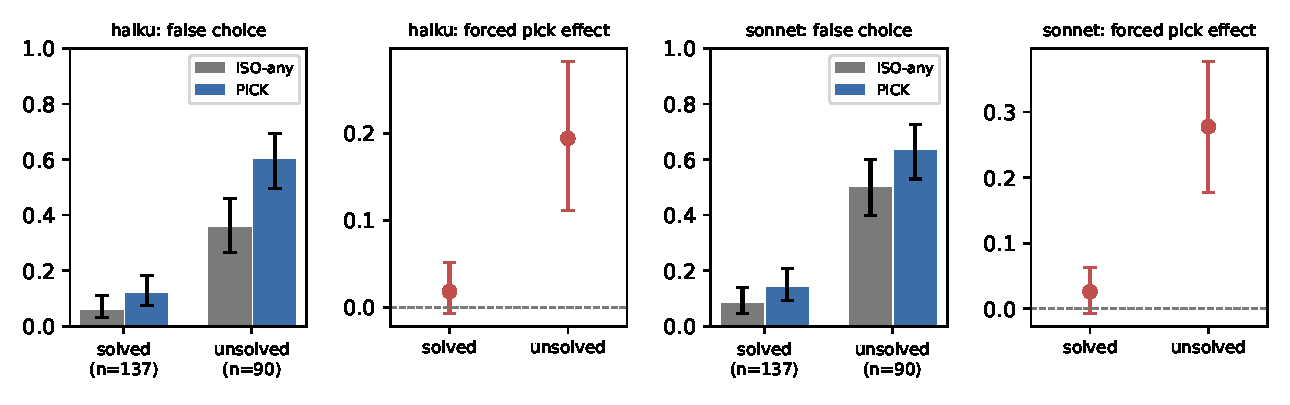
\includegraphics[width=\textwidth]{figures/c3}
\caption{C3. Left of each pair: share of target-absent pools in which the judge chose (PICK) or accepted (ISO-any) a wrong candidate, by haiku stratum, Wilson \res{lvl95} intervals. Right: isolated acceptance of the wrong candidate a forced choice picked minus the mean for the other two, bootstrap \res{lvl95} intervals.}
\label{fig:c3}
\end{figure*}

\subsection{Is it specific to unsolved problems?}
The primary test gave \res{c3h_b} \res{c3h_b_ci} (one-sided $p$ \res{c3h_b_p}, Holm \res{c3h_holm_H1}), which is inconclusive. A permutation test within competition, which needs no error model, agrees (one-sided $p$ \res{rv_h_perm_p}). On the corrected strata the coefficient was \res{all_h_b} \res{all_h_b_ci}. For Sonnet it was \res{c3s_b} \res{c3s_b_ci}. On SOLVED problems, d was also above zero (\res{c3h_ds} \res{c3h_ds_ci}, not a pre-registered test). A significant effect in one stratum does not show the effect is specific to it.

UNSOLVED problems came almost entirely from arXiv-derived sets: contests supplied only \res{c3h_fam_contest_nu} of \res{c3h_fam_contest_n} contest problems to that stratum. Competition fixed effects cannot make up for this lack of overlap. Within the arXiv-derived competitions, which have both strata, haiku's d was \res{rv_h_ov_u} \res{rv_h_ov_u_ci} on \res{rv_h_ov_un} unsolved problems and \res{rv_h_ov_s} \res{rv_h_ov_s_ci} on \res{rv_h_ov_sn} solved ones. Sonnet's was \res{rv_s_ov_u} \res{rv_s_ov_u_ci} and \res{rv_s_ov_s} \res{rv_s_ov_s_ci}. The estimate is above zero on arXiv-derived problems whether or not haiku solved them. These data cannot separate competence from source.

\subsection{Three procedures, one output space}\label{sec:aligned}
Amendment A4 added TP pools and EACH. It pre-registered H4: that $J$ (hit rate minus false-choice rate) is lower for PICK than for ISO on UNSOLVED problems. H4 was not confirmed (\res{a4hu_dj} \res{a4hu_dj_ci} for haiku, \res{a4su_dj} \res{a4su_dj_ci} for Sonnet). Two features of $J$ limit this test. First, an ISO hit required accepting the right candidate and rejecting both wrong ones, which is harder than a PICK hit. Second, $J$ is not a Youden index here, because a hit is one specific candidate while a false choice is any of three. A judge that picks at random whenever it picks has a hit rate of one third of its false-choice rate. So a hit rate equal to the false-choice rate is not chance.

So, post hoc, we gave every procedure the same output: one candidate or abstention. EACH and ISO select at random among the candidates they accepted, scored in expectation, and abstain if they accepted none. Table~\ref{tab:aligned} gives the outcomes. ISO's false choices do not change under this rule. PICK made more correct selections as well as more false choices. For haiku the rise in false choices was larger (\res{al_hpu_pif} \res{al_hpu_pif_ci} against \res{al_hpu_pih} \res{al_hpu_pih_ci}). For Sonnet it was not (\res{al_spu_pif} \res{al_spu_pif_ci} against \res{al_spu_pih} \res{al_spu_pih_ci}). The corrected strata agree (haiku \res{al_hcu_pif} against \res{al_hcu_pih}; Sonnet \res{al_scu_pif} against \res{al_scu_pih}). So for haiku, PICK is not just a shift toward choosing. The pre-registered reading of A4 as a criterion shift rested partly on how an ISO hit was defined. EACH sits between the other two: for haiku, EACH minus ISO in false choice was \res{al_hpu_eif} \res{al_hpu_eif_ci}, and PICK minus EACH was \res{al_hpu_pef} \res{al_hpu_pef_ci}. Seeing candidates together and being asked to choose may both play a part. We did not test these estimates as hypotheses.

The judges could identify a right candidate. When PICK selected on a TP pool, its selection was right in \res{al_hpu_pick_rate} of cases for haiku and \res{al_spu_pick_rate} for Sonnet, against one third by chance. They were much weaker at noticing absence: haiku's PICK selected something in \res{al_hpu_pick_sel} of pools with a right candidate and \res{al_hpu_pick_f} of pools without one. If both pool types were equally common, \res{al_hpu_pick_share} of haiku's PICK selections on these problems would be right. So in this mix a selection helps rank candidates, but is weak evidence that the selected one is right. How weak depends on how often a right candidate is present.

\begin{table*}[t]
\centering\small
\begin{tabular}{llrrrrrr}
\toprule
Judge, UNSOLVED & Procedure & $n$ & False choice & Correct & Wrong & Abstain & Right given selection \\
\midrule
Haiku, pre-registered & PICK & \res{al_hpu_pick_n} & \res{al_hpu_pick_f} & \res{al_hpu_pick_h} & \res{al_hpu_pick_w} & \res{al_hpu_pick_a} & \res{al_hpu_pick_rate} \\
 & EACH & \res{al_hpu_each_n} & \res{al_hpu_each_f} & \res{al_hpu_each_h} & \res{al_hpu_each_w} & \res{al_hpu_each_a} & \res{al_hpu_each_rate} \\
 & ISO & \res{al_hpu_iso_n} & \res{al_hpu_iso_f} & \res{al_hpu_iso_h} & \res{al_hpu_iso_w} & \res{al_hpu_iso_a} & \res{al_hpu_iso_rate} \\
Haiku, corrected & PICK & \res{al_hcu_pick_n} & \res{al_hcu_pick_f} & \res{al_hcu_pick_h} & \res{al_hcu_pick_w} & \res{al_hcu_pick_a} & \res{al_hcu_pick_rate} \\
 & EACH & \res{al_hcu_each_n} & \res{al_hcu_each_f} & \res{al_hcu_each_h} & \res{al_hcu_each_w} & \res{al_hcu_each_a} & \res{al_hcu_each_rate} \\
 & ISO & \res{al_hcu_iso_n} & \res{al_hcu_iso_f} & \res{al_hcu_iso_h} & \res{al_hcu_iso_w} & \res{al_hcu_iso_a} & \res{al_hcu_iso_rate} \\
Sonnet, pre-registered & PICK & \res{al_spu_pick_n} & \res{al_spu_pick_f} & \res{al_spu_pick_h} & \res{al_spu_pick_w} & \res{al_spu_pick_a} & \res{al_spu_pick_rate} \\
 & EACH & \res{al_spu_each_n} & \res{al_spu_each_f} & \res{al_spu_each_h} & \res{al_spu_each_w} & \res{al_spu_each_a} & \res{al_spu_each_rate} \\
 & ISO & \res{al_spu_iso_n} & \res{al_spu_iso_f} & \res{al_spu_iso_h} & \res{al_spu_iso_w} & \res{al_spu_iso_a} & \res{al_spu_iso_rate} \\
Sonnet, corrected & PICK & \res{al_scu_pick_n} & \res{al_scu_pick_f} & \res{al_scu_pick_h} & \res{al_scu_pick_w} & \res{al_scu_pick_a} & \res{al_scu_pick_rate} \\
 & EACH & \res{al_scu_each_n} & \res{al_scu_each_f} & \res{al_scu_each_h} & \res{al_scu_each_w} & \res{al_scu_each_a} & \res{al_scu_each_rate} \\
 & ISO & \res{al_scu_iso_n} & \res{al_scu_iso_f} & \res{al_scu_iso_h} & \res{al_scu_iso_w} & \res{al_scu_iso_a} & \res{al_scu_iso_rate} \\
\bottomrule
\end{tabular}
\caption{One output space (post hoc). False choice is on all-wrong pools. Correct, wrong and abstain are on pools with one right candidate. EACH and ISO select uniformly among accepted candidates, in expectation. Chance for the last column is one third.}
\label{tab:aligned}
\end{table*}

\subsection{Confidence ROC and base rate (A5)}\label{sec:a5}
Amendment A5 asked haiku for a confidence rating (1 to 5) with each PICK and ISO decision. This gives an ROC curve of hit rate against false-choice rate over confidence thresholds (Figure~\ref{fig:roc}). For ISO, we take the candidate with the strictly highest signed confidence if it is positive. A tie gives no identification, and an abstention counts at no threshold. Curves are interpolated linearly from the origin. The partial area runs up to the smaller of the two procedures' maximum false-choice rates, a rule fixed in advance, here \res{a5u_famax}. H6 predicted a smaller area for PICK on UNSOLVED problems. It was not confirmed (\res{a5u_dpauc} \res{a5u_dpauc_ci}). The chance line for this ROC is a hit rate of one third of the false-choice rate (dashed), so both curves lie above chance. The difference between procedures is small and uncertain. H7 asked whether stating that most problems have no correct solution lowers false choices. We could not detect that: \res{a5u_fa_base} with the statement and \res{a5u_fa_pick} without (\res{a5u_dfa} \res{a5u_dfa_ci}).

\begin{figure}[t]
\centering
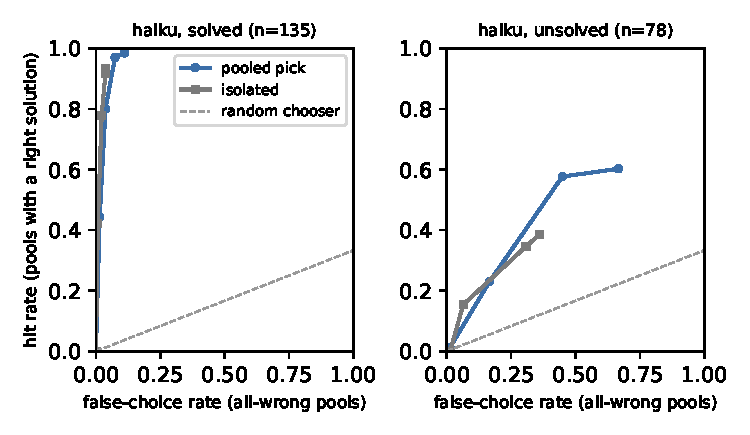
\includegraphics[width=\columnwidth]{figures/roc}
\caption{Lineup ROC for haiku (A5): hit rate on pools with a right candidate against false-choice rate on all-wrong pools, over confidence thresholds. Dashed: a judge that picks uniformly when it picks.}
\label{fig:roc}
\end{figure}

\subsection{Selection and later verification}
H2 tests an association, not a cause. The candidate FORCED picked got an ACCEPT in its single ISO verdict more often than the pool's other wrong candidates. The difference was \res{c3h_h2u} \res{c3h_h2u_ci} on UNSOLVED problems (Holm \res{c3h_holm_H2u}, confirmed) and \res{c3h_h2s} \res{c3h_h2s_ci} on SOLVED (inconclusive). For Sonnet it was \res{c3s_h2u} \res{c3s_h2u_ci} on UNSOLVED. Candidates that look convincing when ranked also look convincing when checked, so this does not show that selection causes a further error. Each candidate has only one verdict, so we do not estimate its acceptance probability. H3 asked whether checking haiku's pick with Sonnet reduces the difference. The reduction was \res{h3_haiku_d} \res{h3_haiku_ci} (inconclusive), and Sonnet accepted the pick in \res{h3_haiku_acc_sonnet} of pools against \res{h3_haiku_acc_haiku} for haiku. The interval does not exclude a moderate reduction. So we failed to detect one, which does not show that cross-model verification fails.

\subsection{Other explanations (post hoc)}\label{sec:checks}
\textbf{Own wrong answer.} A judge may choose a candidate because it matches its own earlier answer. We read both of haiku's solve replies against the candidates of every UNSOLVED pool by hand (exps/c3/own\_answer\_checks.csv; not blind), because automated matching both missed and invented matches. \res{rv_own_with_n} of \res{rv_own_n} pools contained an answer haiku had given. In those pools PICK chose such a candidate in \res{rv_own_pick} selections. For haiku, d was \res{rv_own_with} \res{rv_own_with_ci} with such a candidate and \res{rv_own_wo} \res{rv_own_wo_ci} without one, so the effect is smaller and not clearly above zero without one. This split is not randomised: these pools may also hold more common and more convincing errors. Sonnet, which never saw haiku's replies, also showed \res{rv_own_s_with} \res{rv_own_s_with_ci} and \res{rv_own_s_wo} \res{rv_own_s_wo_ci} on the same split. Recognising its own answer may explain a substantial part of the effect, but these data cannot say how much.
\textbf{Candidate family.} We looked at UNSOLVED pools with both Claude-written and other candidates. FORCED chose a Claude-written one \res{rv_h_cl_obs} times for haiku, against \res{rv_h_cl_exp} expected if blind (of \res{rv_h_cl_n}, $p$ \res{rv_h_cl_p}). For Sonnet it was \res{rv_s_cl_obs} against \res{rv_s_cl_exp} ($p$ \res{rv_s_cl_p}). On SOLVED pools the counts were \res{rv_h_cls_obs} against \res{rv_h_cls_exp} and \res{rv_s_cls_obs} against \res{rv_s_cls_exp}. This could reflect familiar style or simply stronger writing by those models. We cannot tell which. Since \res{rv_claude_share} of candidates are Claude-written, pools built differently could change the size of the main effect.
\textbf{Position.} FORCED picks by position were \res{rv_h_pos} for haiku ($p$ \res{rv_h_pos_p} against a uniform split) and \res{rv_s_pos} for Sonnet ($p$ \res{rv_s_pos_p}). PICK choices were \res{rv_h_posp} and \res{rv_s_posp}. Haiku chooses the middle position less often. Order is shuffled per pool, so this should not favour one kind of candidate, but it was not counterbalanced.
\textbf{Length.} On UNSOLVED problems FORCED chose the longest candidate in \res{rv_h_long} of pools for haiku and \res{rv_s_long} for Sonnet, with one third expected if length were irrelevant and lengths never tied.
\textbf{Compute.} Median output tokens per pool on UNSOLVED problems were \res{rv_h_tok_iso} for ISO and \res{rv_h_tok_pick} for PICK for haiku, and \res{rv_s_tok_iso} and \res{rv_s_tok_pick} for Sonnet. So ISO spends about three times as much, and part of its advantage may come from that. PICK's lower cost should be weighed against its false choices.

\section{Limitations}
\begin{itemize}\setlength{\itemsep}{2pt}
\item \textbf{Procedures, not mechanism.} ISO and PICK differ in calls, context, instruction and how many candidates can pass. So we measure whole procedures.
\item \textbf{Vendor and task.} All interpreted judges are Anthropic models, and all tasks are mathematics with final-answer grading. An open-model arm (gemma-4-e4b, \res{gm_n} problems per stratum, no tests) accepted \res{gm_isowrong} of wrong candidates in isolation. It therefore cannot show a penalty and is uninformative.
\item \textbf{Items.} Pools need three distinct wrong answers, so they are not a random sample. The buildable problems were already used or stratified here, so a fresh holdout needs new MathArena releases.
\item \textbf{Labels.} The two graders shared weaknesses, and MathArena's labels contain errors. Our audits covered the UNSOLVED replies and flagged candidates. They were not blind and were not done by humans.
\item \textbf{Registration.} Plans were committed to a private repository, not a public registry. Their timing rests on repository history and the exported log, which readers cannot fully verify.
\item \textbf{Settings.} Adaptive thinking was not controlled. An answer-only probe was uninformative (\res{cal_haiku_nowork} and \res{cal_sonnet_nowork}), so we cannot exclude contamination of 2025 to 2026 contests. Each verdict is a single sample, so we did not measure variability across repeat runs.
\item \textbf{Missing units.} One haiku EACH reply imitated tool calls instead of answering, and is counted as missing. \res{c3_n_mixed} MIXED problems and one unresolved problem were not judged. An API safeguard blocked three Sonnet calls. Pools remove duplicates by answer string, so two pools hold equivalent wrong answers.
\item \textbf{Primary model.} HC3 errors are undefined for the one competition with a single judged problem. That problem adds nothing to the coefficient, and the reported interval equals the one obtained without it.
\item \textbf{Errors found in review.} A parsing bug changed every earlier solve rate. An external audit led us to recheck our first own-answer analysis, which had an identifier-matching bug and overstated the effect without such candidates. An earlier draft read the ROC diagonal as chance and said a pick carried almost no information. External review corrected this.
\item \textbf{Reviewers.} AI reviewers from two vendors audited this work. They are not independent human validation.
\end{itemize}

\section{Conclusion}
On problems where claude-haiku-5-5's own answers were graded wrong twice, PICK with NONE available produced more false choices on all-wrong pools than ISO did. This held for haiku and for claude-sonnet-5-5, and it survives our audits of strata and labels. The effect is weaker in pools without an answer haiku had given, so recognising one's own error may be part of it. We do not know whether it is specific to problems the judge cannot solve, because the primary test was inconclusive and solvability is entangled with source.

For builders using these two models, we offer three cautions. A NONE option alone did not make a judge reliable at noticing that no candidate is right. A selection is better treated as a ranking than as evidence of correctness. And another model from the same family may not remove the link between selection and verification.

The next experiment should balance solved and unsolved problems within sources, counterbalance candidate order, build pools independently of model name, match compute across ISO, EACH and PICK, repeat verdicts, and add judges from other vendors, on a fresh holdout.

\section*{Data availability and chronology}
The archive holds plans, amendments, prompts, raw replies, grading code, adjudication records and scripts for each table and figure: \url{https://github.com/chaitshar/when-no-candidate-is-correct/tree/v1.0}. It omits verbatim Who\&When logs, which its pinned build script regenerates. MathArena data carry a CC BY-NC-SA licence. Commit hashes below refer to the development repository, which also holds unrelated work and stays private. The archive includes an export of its log. Git commit times, 4 November 2026 UTC: pools locked 08:28 (e11f496c); C3 plan 08:29 (62ab1fc0); first solve data 08:31 (003bd753); Sonnet and H3 amendment 08:36 (7cbaccc2); hand checks 09:10 (ce7eed17); first arm data 09:21 (17818a7f); A4 10:09 (7a11786c); A5 10:53 (b9470c0b). GitHub's event log records a push at 09:10 UTC of commit 12fa20c5, which contains the plan and comes before the first arm data commit (evidence/github/push\_events.json). This limits when the plan could have been written, but does not by itself prove when calls began.

\section*{AI assistance}
The author set the research direction and constraints. An AI system (Claude, via Claude Code) wrote the rules and automated checks at the author's direction. It also ran the search, experiments, analysis and drafting under those rules, and AI agents reviewed the draft. Codex, an OpenAI system, then recomputed the main tables from raw replies with its own code and rechecked the own-answer labels. Its corrections are included. Most of its label disagreements did not survive a recheck against the raw replies. ``Separate'' or ``independent'' agents here means separate AI agents, not humans. The author is responsible for the content. Subject calls cost about \res{cost_subjects} US dollars at list price.

\bibliographystyle{plainnat}
\bibliography{refs}

\appendix
\section{Earlier attempts}\label{app:early}
Earlier banks were interpreted for a model only if its solve rate on them was inside a pre-registered band (\res{band_lo} to \res{band_hi}) and its isolated false-accept rate was above zero. \textbf{Stale items.} On 40 MATH problems with human-verified wrong GPT-4 solutions from PRM800K \citep{lightman2024lets,hendrycks2021measuring}, haiku, sonnet and opus never chose or accepted a wrong candidate in any format (isolated false accept \res{p1_haiku_isowrong}; solve rates \res{p1_haiku_solve}, \res{p1_sonnet_solve}, \res{p1_opus_solve}). These public items sit at the floor and test nothing about current judges; we report them because they were run. Outdated small open models were also run on these pools; under our rules they carry no weight and are listed only in the artifact.

\textbf{Screen.} On 60 screen problems haiku was calibrated (solve rate \res{s1_solve}; isolated accept of wrong candidates \res{s1_isowrong}, that is \res{s1_isowrong_k} of the \res{s1_isowrong_n} distinct wrong candidates, each judged once although some appear in both a TA and a TP pool (\res{s1_wrong_appear} appearances); of right candidates \res{s1_isoright}). The TA choosing rate was \res{s1_ta_iso} for ISO, \res{s1_ta_pick} for PICK and \res{s1_ta_each} for EACH (Figure~\ref{fig:lineup}). PICK minus ISO was \res{s1_pickiso} \res{s1_pickiso_ci}; PICK minus EACH \res{s1_pickeach} \res{s1_pickeach_ci}. With a right candidate present, PICK chose a wrong one in \res{s1_tp_pick_false} of pools, against \res{s1_tp_iso_false} in which isolated verification accepted at least one wrong candidate; this comparison favours PICK by construction (PICK can choose at most one candidate, ISO-any can accept several) and is descriptive only.

\begin{figure*}[t]
\centering
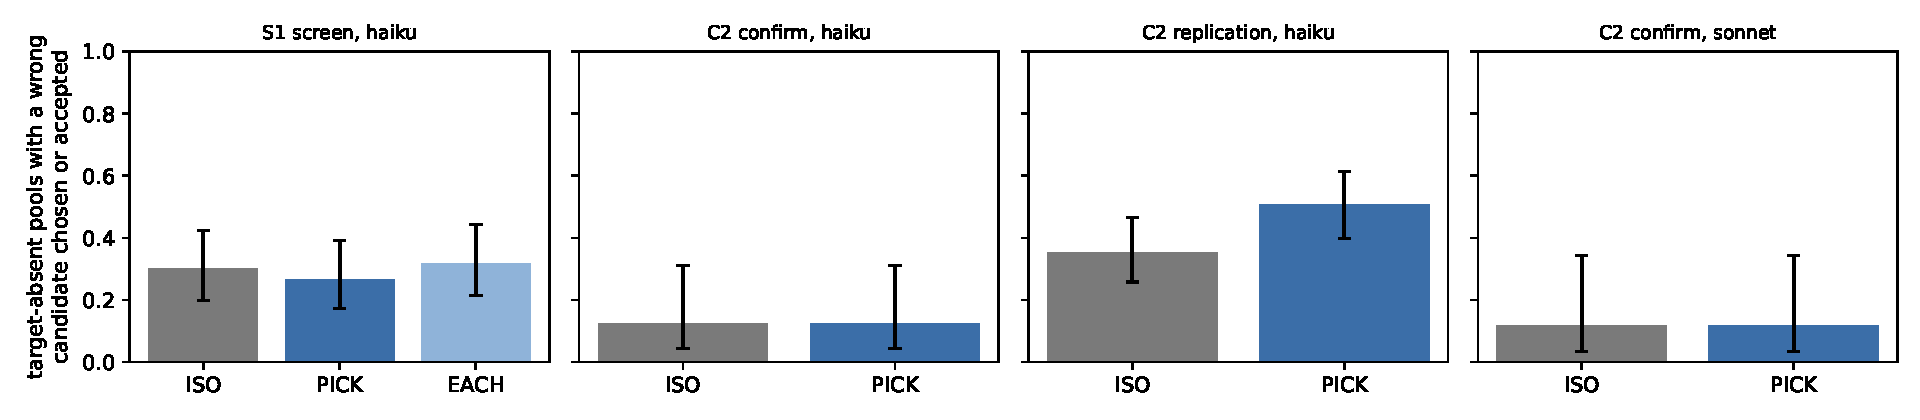
\includegraphics[width=\textwidth]{figures/lineup}
\caption{Share of target-absent pools in which the judge chose (PICK) or accepted (ISO, any of three isolated calls; EACH) a wrong candidate, with Wilson \res{lvl95} intervals. Panels: screen and pre-registered held-out sets.}
\label{fig:lineup}
\end{figure*}

\textbf{Uninterpretable confirmation (C2).} Pools came from HMMT February and AIME 2026 and arXiv-math August and September 2026. C2 pre-registered H1 (equivalence of PICK and ISO-any within $\pm$\res{eq_margin}), H2 (select then verify, below) and a calibration gate ``per model and set''. A review found that our answer parser dropped a leading LaTeX dollar and backslash, so some correct solutions were graded wrong; with the parser fixed (exps/c2\_confirm/AMENDMENTS.md A3), haiku solved \res{c2_haiku_conf_solve} of the 2026 contest problems, above the band, and \res{c2_haiku_repl_solve} of the arXiv-derived problems, below it. The union of both sets falls inside the band only by pooling (\res{c2_haiku_all_solve}); following our conservative ruling for such conflicts (made after the data, AMENDMENTS A2), the union is not interpretable either. C2 therefore tests nothing for haiku. For completeness: on the contest set H1 gave \res{c2_haiku_conf_h1d} \res{c2_haiku_conf_h1ci90} and H2 \res{c2_haiku_conf_h2}; on the union H1 \res{c2_haiku_all_h1d} \res{c2_haiku_all_h1ci90} and H2 \res{c2_haiku_all_h2} \res{c2_haiku_all_h2ci}; on the arXiv-derived set H1 \res{c2_haiku_repl_h1d} and H2 \res{c2_repl_h2}. Sonnet failed its gate (isolated-verdict parse rate \res{c2_sonnet_isoparse}, below the pre-registered threshold).

A post hoc split over the screen and C2 problems suggested the penalty sits on problems the judge cannot solve (\res{ph_unsolved_d} versus \res{ph_solved_d}), but solvability then rested on one attempt and one grader with a known bug, and was confounded with source. C3 was designed to test this properly.

\section{Exploratory screens}
These are screens, never findings; each had a written kill rule. \textbf{Failure attribution (Who\&When).} Agent-level accuracy was \res{s5_haiku_agent} (haiku) and \res{s5_sonnet_agent} (sonnet) with strict name matching, \res{s5_haiku_agentnorm} and \res{s5_sonnet_agentnorm} after a post hoc name normalization; step-level accuracy \res{s5_haiku_step} and \res{s5_sonnet_step}. On hand-crafted logs, always naming the most frequent agent scores \res{s5_hand_majority}; normalized accuracy was \res{s5_haiku_handnorm} (haiku, below it) and \res{s5_sonnet_handnorm} (sonnet, close to it). \textbf{Critiques.} A false critique (``the final answer is wrong'') lowered acceptance of right candidates by \res{s4_right_checker} \res{s4_right_checker_ci} when attributed to an automated checker and by \res{s4_right_student} \res{s4_right_student_ci} when attributed to another student. \textbf{Debate with both sides wrong.} A haiku judge who saw only the debate answered NEITHER in \res{s8_ta_neither} of TA pairs and chose the right side in \res{s8_tp_right} of TP pairs. \textbf{Peer notes.} A wrong answer left by ``another agent'' changed haiku's accuracy by \res{s9_wrong_diff} \res{s9_wrong_ci}, adopted in \res{s9_adopt} of problems. \textbf{Agreement and diversity (MathArena's own runs, no subject calls).} For the \res{s2_n_big} models with at least 60 problems, the AUROC of self-consistency agreement ranged \res{s2_auroc_min} to \res{s2_auroc_max} and unanimous answers were wrong at most \res{s2_unan_wrong_max}; errors correlated less across different models (phi \res{s10_hetero}) than across samples of one model (\res{s10_homo}). \textbf{Tournaments.} In a round-robin of forced pairwise comparisons (haiku, 40 problems), a unique winner emerged in \res{s3_ta_unique} of TA pools and a unanimous one in \res{s3_ta_unan}. The tournament's decisiveness separated TP from TA pools with AUROC \res{s3_auroc} \res{s3_auroc_ci}, so its own statistics give little warning that every candidate is wrong. A pilot on the stale items gave AUROC \res{p2_haiku_auroc} (haiku) and \res{p2_sonnet_auroc} (sonnet), even though those judges rejected every such candidate in isolation. A forced pick in the screen was accepted by haiku's isolated verification in \res{s6_picked} of pools, against \res{s6_unpicked} for the other candidates (\res{s6_diff}, \res{s6_ci}); this motivated H2.

\begin{figure}[t]
\centering
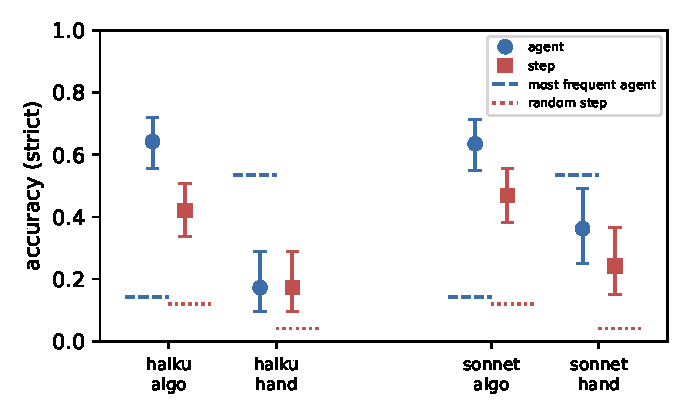
\includegraphics[width=\columnwidth]{figures/whowhen}
\caption{Who\&When attribution accuracy (strict), agent (circles) and step (squares), Wilson \res{lvl95} intervals; dashed line: always naming the most frequent labelled agent (agent baseline); dotted line: a uniformly random step (step baseline).}
\label{fig:ww}
\end{figure}

\end{document}
